\documentclass[11pt,a4paper]{article}
\usepackage{amsmath,amssymb}
\usepackage[margin=2.5cm]{geometry}
\usepackage{array}
\usepackage{bm}
\usepackage{graphicx}
\usepackage{booktabs}
\usepackage{xcolor}
\usepackage{tikz}
\usetikzlibrary{arrows.meta,positioning,fit,backgrounds,calc}
\usepackage{hyperref}
\hypersetup{colorlinks=true, linkcolor=blue!50!black, citecolor=blue!50!black, urlcolor=blue!50!black}

% ---- tikz styles ----
\tikzset{
  block/.style={rectangle, rounded corners, draw=black!60, fill=blue!6,
    minimum height=9mm, minimum width=22mm, align=center, font=\small},
  frozen/.style={rectangle, rounded corners, draw=black!50, fill=black!7,
    minimum height=9mm, minimum width=22mm, align=center, font=\small},
  learn/.style={rectangle, rounded corners, draw=blue!60!black, fill=blue!14, very thick,
    minimum height=9mm, minimum width=22mm, align=center, font=\small},
  io/.style={rectangle, draw=black!40, fill=yellow!10, minimum height=8mm, align=center, font=\small},
  arr/.style={-{Stealth[length=2.2mm]}, thick},
}

\title{\textbf{Flow-Conditioned Metric 3D Point Tracking}\\[2pt]
\large Optical flow $+$ metric depth $+$ a DINOv3-conditioned Mamba-3 depth refiner}
\author{Masahiro Ogawa}
\date{\today}

\begin{document}
\maketitle

\begin{abstract}
We address tracking query points in \emph{metric} 3D across a monocular video, where the
quantity that ultimately governs real-world accuracy is the per-point depth. Rather than learning
tracking end-to-end, we compose two frozen, well-understood front-ends --- dense optical
flow~\cite{searaft,waft} for 2D correspondence and a monocular metric-depth
network~\cite{da3} for the third dimension --- and learn only the residual they cannot supply:
the depth along each point's (fixed) pixel ray, refined by a tiny causal Mamba-3 state-space
model~\cite{mamba3} conditioned on DINOv3~\cite{dinov3} appearance features. This isolates the
single degree of freedom that determines 3D error, while keeping the model small ($\sim$0.5\,M
parameters) and the pipeline interpretable.
On the TAPVid-3D~\cite{tapvid3d} minival benchmark, our best configuration (WAFT flow $+$
Depth-Anything-3 depth $+$ the DINOv3-conditioned refiner) attains the highest \emph{absolute}
metric accuracy of all methods evaluated under identical conditions --- mean metric-AJ $0.246$,
ahead of strong feed-forward 3D trackers --- confirming that a targeted depth-only refinement
recovers real-world 3D structure that scale-invariant training leaves on the table. To measure
this we introduce an absolute-metric evaluation protocol that scores error at fixed metre
thresholds, exposing depth quality that the standard scale-invariant leaderboard metric hides.
A companion reliability analysis --- reproduced with each competitor's own official evaluator ---
explains why several published 3D trackers collapse under a fixed monocular, single-GPU budget,
separating genuine method limitations from evaluation artefacts.
\end{abstract}

\tableofcontents

% =====================================================================
\section{Method}

\subsection{Overview}
Given a video $\{I_t\}_{t=1}^{F}$ and query points $\{(\mathbf{u}_n, a_n)\}_{n=1}^{N}$ (pixel
position $\mathbf{u}_n$ at anchor frame $a_n$), the goal is a 3D track
$\hat{\mathbf X}\in\mathbb{R}^{F\times N\times 3}$ and visibility $\hat v\in\{0,1\}^{F\times N}$.
Our pipeline (Fig.~\ref{fig:pipeline}) has a \emph{training-free} baseline --- SEA-RAFT
flow-chaining for the 2D track plus DA3 unprojection for 3D --- and a small \emph{learned} module,
v33, that refines depth.

\begin{figure}[h]
\centering
\resizebox{\textwidth}{!}{%
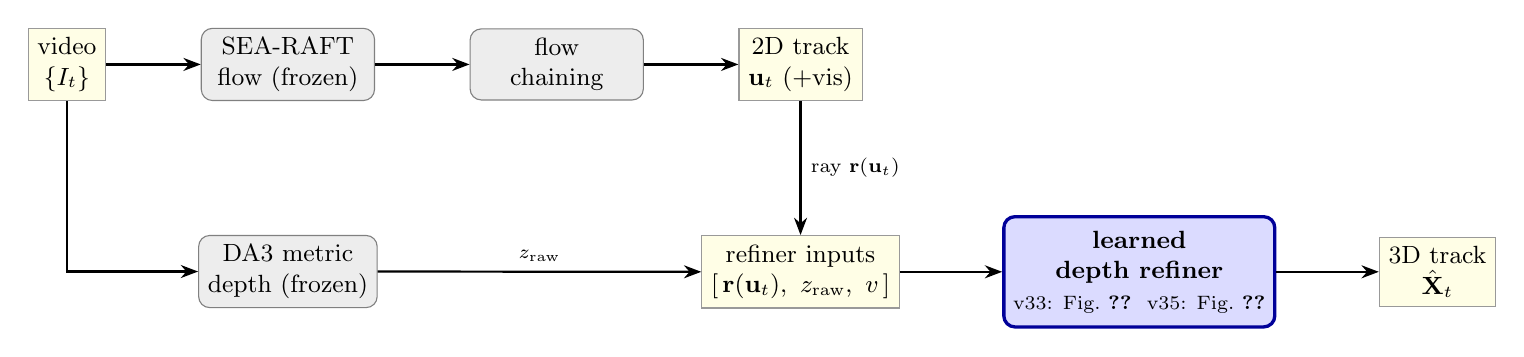
\begin{tikzpicture}[node distance=9mm and 12mm]
  \node[io] (vid) {video\\$\{I_t\}$};
  \node[frozen, right=of vid] (flow) {SEA-RAFT\\flow (frozen)};
  \node[frozen, right=of flow] (chain) {flow\\chaining};
  \node[io, right=of chain] (uv) {2D track\\$\mathbf{u}_t$ (+vis)};
  \node[frozen, below=17mm of flow] (da3) {DA3 metric\\depth (frozen)};
  % refiner inputs (yellow) — the SAME yellow input box as Fig 3 / Fig 5.
  \node[io, below=17mm of uv] (inp) {refiner inputs\\$[\,\mathbf{r}(\mathbf{u}_t),\ z_{\text{raw}},\ v\,]$};
  % the single learned module (large blue box); internals in Fig 3 / Fig 5.
  \node[learn, minimum width=30mm, minimum height=14mm, right=13mm of inp] (ref)
    {\textbf{learned}\\\textbf{depth refiner}\\{\scriptsize v33: Fig.~\ref{fig:arch}\ \ v35: Fig.~\ref{fig:v35-arch}}};
  \node[io, right=13mm of ref] (out) {3D track\\$\hat{\mathbf X}_t$};

  \draw[arr] (vid) -- (flow);
  \draw[arr] (flow) -- (chain);
  \draw[arr] (chain) -- (uv);
  \draw[arr] (vid.south) |- (da3.west);
  \draw[arr] (uv) -- (inp) node[midway, right, font=\scriptsize] {ray $\mathbf{r}(\mathbf{u}_t)$};
  \draw[arr] (da3.east) -- (inp.west) node[midway, above, font=\scriptsize] {$z_{\text{raw}}$};
  \draw[arr] (inp) -- (ref);
  \draw[arr] (ref) -- (out);
\end{tikzpicture}%
}
\caption{Overall pipeline. Grey = frozen / training-free; the \textbf{large blue box} is the only
learned module ($0.40$M params); its internals are Fig.~\ref{fig:arch} (v33) and
Fig.~\ref{fig:v35-arch} (v35). SEA-RAFT's 2D track $\mathbf{u}_t$ (and visibility) are \emph{never}
modified. The refiner's \emph{inputs} (yellow box) --- the frozen pixel ray $\mathbf{r}(\mathbf{u}_t)$
(from $\mathbf{u}_t$ and the intrinsics), DA3's raw depth $z_{\text{raw}}$, and visibility $v$ --- are
exactly the yellow input boxes that sit \emph{outside} the blue box in Fig.~\ref{fig:arch} and
Fig.~\ref{fig:v35-arch} (v35 additionally feeds a $5{\times}5$ depth patch and a DINOv3 feature). The
box corrects depth along the frozen ray and unprojects to 3D, so the 2D reprojection is invariant by
construction (Fig.~\ref{fig:ray}).}
\label{fig:pipeline}
\end{figure}

\subsection{2D track: SEA-RAFT flow-chaining (baseline, frozen)}
We precompute dense forward/backward flow for consecutive frames with a frozen SEA-RAFT model,
$\mathbf{f}^{\rightarrow}_t,\mathbf{f}^{\leftarrow}_t$. Each query is propagated outward from its
anchor by bilinearly sampling the flow at the current position,
\begin{equation}
\mathbf{u}_{t+1} = \mathbf{u}_t + \mathcal{S}\!\left(\mathbf{f}^{\rightarrow}_t,\,\mathbf{u}_t\right),
\qquad
\mathbf{u}_{t-1} = \mathbf{u}_t + \mathcal{S}\!\left(\mathbf{f}^{\leftarrow}_{t-1},\,\mathbf{u}_t\right),
\end{equation}
where $\mathcal{S}$ is bilinear sampling. Visibility uses a forward--backward consistency test:
a hop is consistent iff $\lVert \mathbf{d}^{\rightarrow}+\mathbf{d}^{\leftarrow}\rVert \le
\alpha\,(\lVert\mathbf{d}^{\rightarrow}\rVert+\lVert\mathbf{d}^{\leftarrow}\rVert)+\beta$
($\alpha{=}0.05$, $\beta{=}1$\,px), and a point stays occluded once it fails. This 2D track is
strong on its own and is held \emph{fixed} for everything downstream.

\subsection{Metric depth and differentiable unprojection}
DA3 supplies a per-frame metric depth map $D_t$ (absolute metres). We sample it at the tracked
pixel and unproject with the pinhole intrinsics $K=(f_x,f_y,c_x,c_y)$:
\begin{equation}
z_t = \mathcal{S}(D_t,\mathbf{u}_t),\qquad
\hat{\mathbf X}_t = \Big(\tfrac{u_t-c_x}{f_x}\,z_t,\;\tfrac{v_t-c_y}{f_y}\,z_t,\;z_t\Big).
\label{eq:unproject}
\end{equation}
Sampling is done with \texttt{grid\_sample} so gradients flow to the (refined) depth; the depth
model itself is frozen. The baseline \emph{SEA-RAFT$+$DA3} tracker is exactly
Eq.~\eqref{eq:unproject} with $z_t$ taken directly from DA3.

\subsection{v33: Mamba-3 depth-along-ray refiner (the method)}
DA3 metric depth is accurate in \emph{relative} structure but carries a global scale bias
(e.g.\ $\sim$40\% on far-field driving scenes). v33 learns a small temporal correction to the
depth, leaving the 2D track untouched. The key design choice: with the pixel $\mathbf{u}_t$ frozen,
the only 3D degree of freedom that preserves the 2D reprojection is the depth $z_t$ along the pixel
ray (Fig.~\ref{fig:ray}).

\begin{figure}[h]
\centering
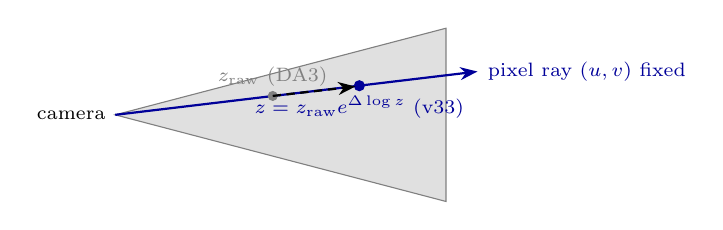
\begin{tikzpicture}[scale=1.0]
  \coordinate (cam) at (0,0);
  \draw[fill=black!12,draw=black!50] (cam) -- (4.2,1.1) -- (4.2,-1.1) -- cycle;
  \node[font=\scriptsize,left] at (cam) {camera};
  \draw[arr,blue!60!black,thick] (cam) -- (4.6,0.55) node[right,font=\scriptsize]{pixel ray $(u,v)$ fixed};
  \filldraw[gray] (2.0,0.24) circle (1.6pt) node[above,font=\scriptsize]{$z_{\text{raw}}$ (DA3)};
  \filldraw[blue!60!black] (3.1,0.37) circle (1.8pt) node[below,font=\scriptsize]{$z=z_{\text{raw}}e^{\Delta\log z}$ (v33)};
  \draw[arr,densely dashed] (2.0,0.24) -- (3.05,0.36);
\end{tikzpicture}
\caption{Depth-along-ray refinement. The tracked pixel (hence the ray direction) is frozen, so
\emph{only the depth slides along the ray} and the 2D projection is unchanged: v33 moves the point's
depth alone, leaving the predicted 2D track and visibility invariant.}
\label{fig:ray}
\end{figure}

\paragraph{Inputs and architecture.} For each track $n$ and frame $t$ the SSM receives a $4$-D
feature: the normalised ray direction $\big(\tfrac{u-c_x}{f_x},\tfrac{v-c_y}{f_y}\big)$,
the depth ratio $z_{\text{raw}}/z_{\text{ref}}$ ($z_{\text{ref}}=$ per-clip median depth), and
the visibility flag.  The SSM \emph{does not see $z_{\text{raw}}$ directly}; it only sees the
scale-normalised ratio.  This is a deliberate training-stability choice: DA3 depths span
$\sim$1\,m (\emph{adt}) to $\sim$20\,m (\emph{drivetrack}), and an unnormalised input would
require the same network weights to operate across a 20$\times$ dynamic range.

The SSM's role is therefore to predict a \emph{relative} correction factor, not an absolute
depth.  $z_{\text{raw}}$ bypasses the SSM entirely and is multiplied back in outside the learned
module (Fig.~\ref{fig:arch}):
\begin{equation}
\Delta\log z_t = \mathrm{clamp}\big(\mathrm{head}(h_t),\,\pm 2\big),\qquad
z_t = z_{\text{raw},t}\cdot e^{\Delta\log z_t}.
\label{eq:correction}
\end{equation}
Because the SSM never sees the absolute scale, it cannot reason about it directly; any
global-scale correction it learns must be inferred indirectly from temporal and structural
patterns in the normalised input (e.g.\ the characteristic depth-change profile of a driving
scene vs.\ an indoor one).  A natural future improvement is to also feed $\log z_{\text{ref}}$
as a scalar context token, giving the SSM direct access to the clip-level scale without
sacrificing the per-point normalisation.

Zero-initialising the head means v33 starts exactly at the SEA-RAFT$+$DA3 baseline and only
learns improvements.  The model has $\approx0.40$M trainable parameters.

\begin{figure}[h]
\centering
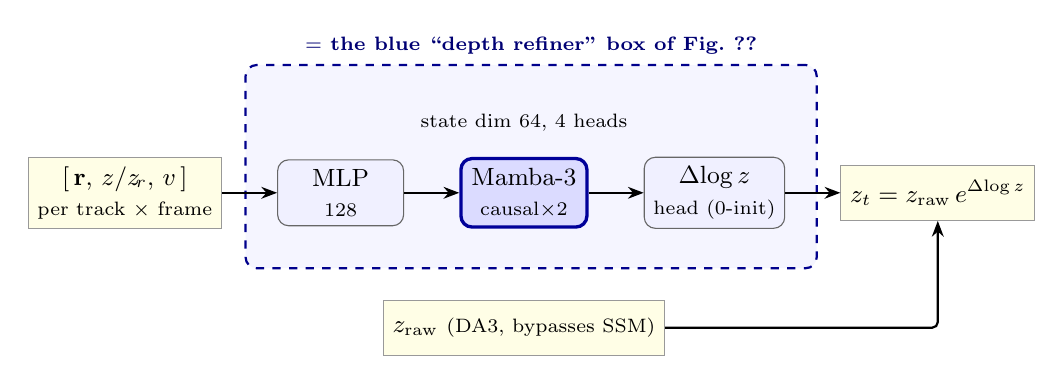
\begin{tikzpicture}[
    node distance=4mm and 7mm,
    block/.style={rectangle, rounded corners, draw=black!60, fill=blue!6,
      minimum height=8mm, minimum width=16mm, align=center, font=\small},
    frozen/.style={rectangle, rounded corners, draw=black!50, fill=black!7,
      minimum height=8mm, minimum width=16mm, align=center, font=\small},
    learn/.style={rectangle, rounded corners, draw=blue!60!black, fill=blue!14, very thick,
      minimum height=8mm, minimum width=16mm, align=center, font=\small},
    io/.style={rectangle, draw=black!40, fill=yellow!10,
      minimum height=7mm, align=center, font=\small},
    arr/.style={-{Stealth[length=2mm]}, thick},
  ]
  % SSM path (top row)
  \node[io] (in) {$[\,\mathbf{r},\,z/z_{\!r},\,v\,]$\\{\scriptsize per track $\times$ frame}};
  \node[block, right=of in] (emb) {MLP\\{\scriptsize 128}};
  \node[learn, right=of emb] (m1) {Mamba-3\\{\scriptsize causal$\times$2}};
  \node[block, right=of m1] (head) {$\Delta\!\log z$\\{\scriptsize head (0-init)}};
  \node[io, right=of head] (z) {$z_t = z_{\text{raw}}\,e^{\Delta\!\log z}$};
  % z_raw bypass (below)
  \node[io, below=9mm of m1] (zraw) {$z_{\text{raw}}$ {\scriptsize (DA3, bypasses SSM)}};
  % Arrows: SSM path
  \draw[arr] (in) -- (emb);
  \draw[arr] (emb) -- (m1);
  \draw[arr] (m1) -- (head);
  \draw[arr] (head) -- (z);
  % z_raw bypass arrow: right from zraw.east, then up into z.south (short L).
  \draw[arr,rounded corners=2pt] (zraw.east) -- (zraw.east -| z.south) -- (z.south);
  \node[font=\scriptsize, above=2mm of m1, align=center] (ann)
    {state dim 64, 4 heads};
  % Blue container wraps ONLY the learned internals; the yellow I/O boxes (input, z_t,
  % z_raw bypass) sit OUTSIDE it — they cross the boundary of the blue box of Fig 1.
  \begin{scope}[on background layer]
    \node[draw=blue!55!black, dashed, thick, rounded corners, fill=blue!4,
          fit=(emb)(m1)(head)(ann), inner sep=4mm, inner ysep=5mm,
          label={[font=\scriptsize\bfseries, blue!45!black]above:{$=$ the blue ``depth refiner'' box of Fig.~\ref{fig:pipeline}}}] {};
  \end{scope}
\end{tikzpicture}
\caption{v33 architecture --- the inside of the blue box in Fig.~\ref{fig:pipeline}.
Input abbreviations: $\mathbf{r}{=}(\text{ray}_x,\text{ray}_y)$ is the frozen pixel ray from the 2D
track $\mathbf{u}_t$,
$z/z_{\!r}{=}z_{\text{raw}}/z_{\text{ref}}$, $v{=}$visibility.
\textbf{Bypass}: $z_{\text{raw}}$ (DA3 metric depth) skips the SSM entirely and is multiplied
back in at the end — the SSM is a \emph{relative corrector} that predicts the factor
$e^{\Delta\log z}$, not an absolute depth.
\textbf{causal$\times$2}: two causal Mamba-3 layers (past-only; enables streaming).
\textbf{4 heads}: SSD splits the 64-dim state into 4 independent heads (16-dim each), analogous
to multi-head attention but computed as a linear recurrence.}
\label{fig:arch}
\end{figure}

\subsection{Why depth-only (and not 2D)}
An earlier variant (v32) added a learned 2D residual $\Delta\mathbf{u}$ on top of SEA-RAFT. It
\emph{degraded} accuracy: SEA-RAFT's 2D track is already near-optimal, and small nudges push the
sampling location across DA3 depth discontinuities (object boundaries), flipping points out of the
correctness band. v33 therefore freezes the 2D track entirely and refines depth only --- the lever
that actually carries the error.

% -----------------------------------------------------------------------
\subsection{v35: image-conditioned joint 2D--depth refiner}
\label{sec:v35}

v35 revisits the joint 2D--depth correction that failed in v32, but removes its root cause.
v32 nudged the pixel blindly; the SSM had no way to tell whether it was pushing toward or
away from a depth discontinuity.
v35 gives it that context through two new per-track inputs:

\begin{itemize}
\item \textbf{DINOv3 appearance features} (64-D): sampled from a frozen ViT-S/16
  \emph{DINOv3}~\cite{dinov3} backbone (\texttt{dinov3-vits16-pretrain-lvd1689m}) at the current
  track position. These provide a local visual ``fingerprint'' of the tracked object, allowing the
  SSM to detect when the 2D position has drifted off the target.
  We use DINOv3 rather than DINOv2 specifically for its \emph{dense} (patch-level) features. DINOv3
  is Meta's 2025 self-supervised ViT, trained on ${\sim}1.7$B images (LVD-1689M, ${\sim}12\times$
  DINOv2's 142M) with a \emph{Gram-anchoring} loss that keeps the patch-token feature map sharp and
  spatially consistent throughout the long training schedule --- DINOv2's dense features, by
  contrast, degrade as pre-training progresses. Since we sample a single feature vector at each
  track pixel, this patch-level fidelity is exactly what matters, so DINOv3's dense maps are a
  better fit than DINOv2's here. (The encoder class in our code is still named \texttt{DINOv2Encoder}
  for legacy reasons, but it loads the DINOv3 weights above.)
\item \textbf{Local depth patch} (25 values). We read the DA3 depth at a $5{\times}5$ grid of points
  centred on the tracked pixel $\mathbf{u}_0$: 25 points in total, each one bilinearly-interpolated
  depth value. Along each axis the five points sit at offsets
  $\{-2,-1,0,1,2\}\times(\text{image\_size}/14)$ pixels from $\mathbf{u}_0$, so the grid spacing and
  extent scale with the input size. \emph{Concretely, for our $896$-px inputs} the spacing is
  $896/14 = 64$\,px: the five offsets are $\{-128,-64,0,+64,+128\}$\,px, so the grid spans a
  $256{\times}256$-px window around the point. We then divide all 25 depths by the depth at the
  \emph{centre} point, giving 25 scale-invariant depth \emph{ratios} (the centre ratio is exactly
  $1$), and concatenate all 25 into the SSM input. Passing ratios rather than raw depths lets the SSM
  read local depth \emph{structure} --- the relative jumps that mark object boundaries --- independent
  of how far away the point is; this is the depth-discontinuity cue that v32 lacked and overshot
  without.
\end{itemize}

A second output head (also zero-initialised) predicts a 2D correction $\Delta\mathbf{u}$. Its raw
output is passed through a $\tanh$ (which limits it to $[-1,1]$) and then scaled by $2$, i.e.\
$\Delta\mathbf{u} = 2\tanh(\cdot)$, so the pixel can shift by at most $\pm 2$\,px.
Crucially, after $\Delta\mathbf{u}$ shifts the pixel,
depth is \emph{re-sampled} at the corrected position from the DA3 depth map before
$\Delta\!\log z$ is applied.  This ensures the depth and 2D corrections remain geometrically
consistent (Fig.~\ref{fig:v35-concept}).

\begin{figure}[h]
\centering
\resizebox{\textwidth}{!}{%
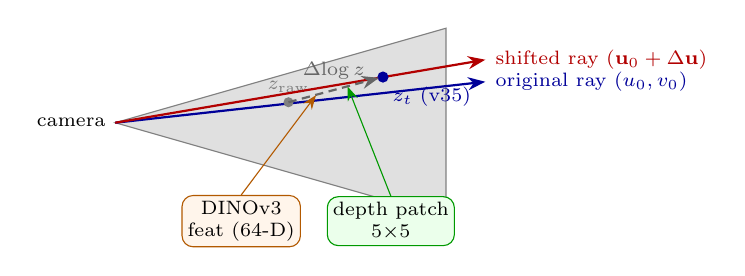
\begin{tikzpicture}[scale=1.0]
  \coordinate (cam) at (0,0);
  \draw[fill=black!12,draw=black!50] (cam) -- (4.2,1.2) -- (4.2,-1.2) -- cycle;
  \node[font=\scriptsize,left] at (cam) {camera};
  % original SEA-RAFT ray
  \draw[arr,blue!60!black,thick] (cam) -- (4.7,0.52)
    node[right,font=\scriptsize,blue!60!black]{original ray $(u_0,v_0)$};
  \filldraw[gray] (2.2,0.26) circle (1.6pt) node[above,font=\scriptsize,gray]{$z_{\rm raw}$};
  % new ray after Δu
  \draw[arr,red!70!black,thick] (cam) -- (4.7,0.80)
    node[right,font=\scriptsize,red!70!black]{shifted ray $(\mathbf{u}_0+\Delta\mathbf{u})$};
  % v35 corrected point: Δlog_z along new ray
  \filldraw[blue!60!black] (3.4,0.58) circle (1.8pt)
    node[below right,font=\scriptsize,blue!60!black]{$z_t$ (v35)};
  \draw[arr,densely dashed,black!60] (2.2,0.26) -- (3.35,0.57)
    node[midway,above,font=\scriptsize]{$\Delta\!\log z$};
  % DINOv3 and depth-patch inputs: spaced apart, both pointing to the Δlog z correction arrow.
  \node[draw=orange!70!black,fill=orange!8,rounded corners,font=\scriptsize,inner sep=2pt,align=center]
    (dinobox) at (1.6,-1.25) {DINOv3\\feat (64-D)};
  \draw[-{Stealth[length=1.8mm]},orange!70!black] (dinobox.north) -- (2.55,0.35);
  \node[draw=green!60!black,fill=green!8,rounded corners,font=\scriptsize,inner sep=2pt,align=center]
    (patchbox) at (3.5,-1.25) {depth patch\\$5{\times}5$};
  \draw[-{Stealth[length=1.8mm]},green!60!black] (patchbox.north) -- (2.95,0.46);
\end{tikzpicture}%
}
\caption{v35 joint correction. Two new inputs --- the DINOv3 appearance feature (orange) and a local
$5{\times}5$ depth patch (green) --- give the model the context to predict a 2D shift $\Delta\mathbf{u}$
safely. Unlike v32, which nudged the pixel blindly and crossed depth discontinuities, v35's 2D
correction is conditioned on local appearance and local depth structure, so the informed
$\Delta\mathbf{u}$ avoids depth-discontinuity artefacts. Depth is then re-sampled at the shifted pixel
$\mathbf{u}_0{+}\Delta\mathbf{u}$ before $e^{\Delta\!\log z}$ rescales it.}
\label{fig:v35-concept}
\end{figure}

\begin{figure}[h]
\centering
\resizebox{\textwidth}{!}{%
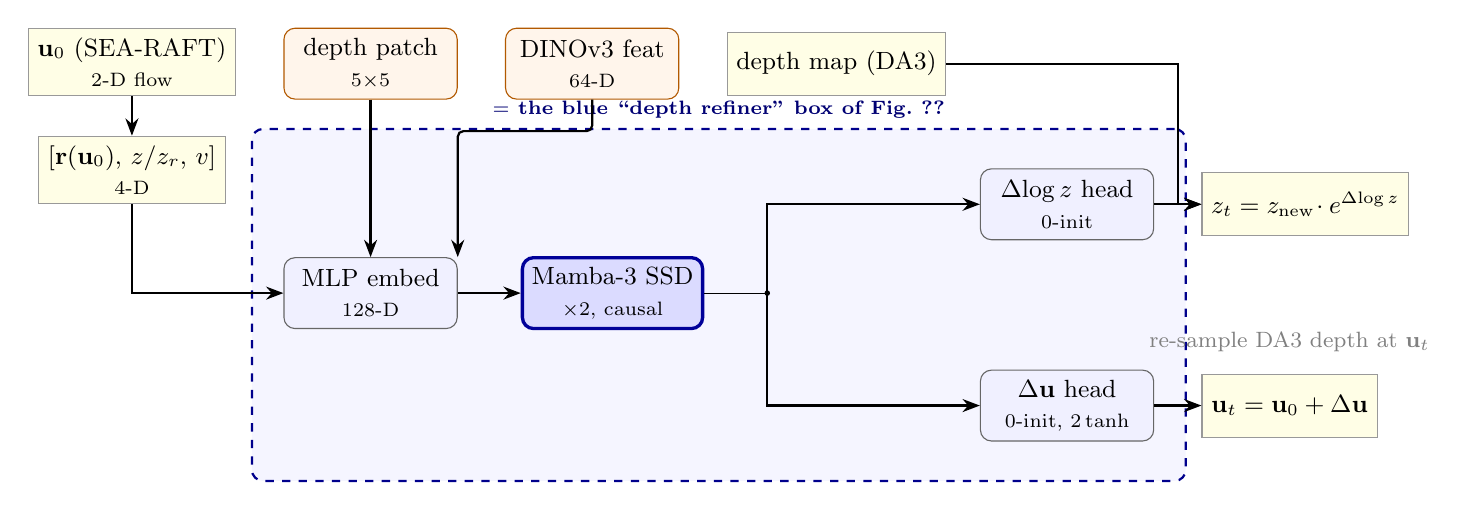
\begin{tikzpicture}[
    node distance=4mm and 6mm,
    new/.style={rectangle, rounded corners, draw=orange!70!black, fill=orange!8,
      minimum height=9mm, minimum width=22mm, align=center, font=\small},
  ]
  % ── inputs (top row): patch and dino as anchors ───────────────────
  \node[new] (patch) {depth patch\\{\scriptsize $5{\times}5$}};
  \node[new, right=6mm of patch] (dino) {DINOv3 feat\\{\scriptsize 64-D}};
  % u0 top-aligned with depth patch; r(u0) stacked below
  \node[io, anchor=north east] (uv0) at ($(patch.north west)+(-6mm,0)$)
    {$\mathbf{u}_0$ (SEA-RAFT)\\{\scriptsize 2-D flow}};
  \node[io, below=5mm of uv0] (in1) {$[\mathbf{r}(\mathbf{u}_0),\,z/z_r,\,v]$\\{\scriptsize 4-D}};
  % depth map: same row as depth patch
  \node[io, right=6mm of dino] (dm) {depth map (DA3)};
  % ── embed ─────────────────────────────────────────────────────────
  \node[block, below=20mm of patch] (emb) {MLP embed\\{\scriptsize 128-D}};
  % ── SSM ───────────────────────────────────────────────────────────
  \node[learn, right=8mm of emb] (ssm) {Mamba-3 SSD\\{\scriptsize $\times 2$, causal}};
  % ── output heads ($\Delta\!\log z$ upper, $\Delta\mathbf{u}$ lower) ─
  \node[block, above right=2mm and 35mm of ssm] (dz)  {$\Delta\!\log z$~head\\{\scriptsize 0-init}};
  \node[block, below right=5mm and 35mm of ssm] (duv) {$\Delta\mathbf{u}$~head\\{\scriptsize 0-init, $2\tanh$}};
  % ── outputs ───────────────────────────────────────────────────────
  \node[io, right=6mm of dz]  (zout)  {$z_t = z_{\rm new}\!\cdot e^{\Delta\!\log z}$};
  \node[io, right=6mm of duv] (uvout) {$\mathbf{u}_t = \mathbf{u}_0+\Delta\mathbf{u}$};
  % ── arrows ────────────────────────────────────────────────────────
  \draw[arr] (uv0) -- (in1);
  \draw[arr] (in1.south) |- (emb.west);
  \draw[arr] (patch.south) -- (emb.north);
  \draw[arr,rounded corners=2pt] (dino.south) -- ++(0,-4mm) coordinate (aux)
    -- (aux -| emb.north east) -- (emb.north east);
  \draw[arr] (emb) -- (ssm);
  \coordinate (ssmfork) at ($(ssm.east)+(8mm,0)$);
  \draw (ssm.east) -- (ssmfork);
  \fill (ssmfork) circle[radius=1pt];
  \draw[arr] (ssmfork) -- (ssmfork |- dz.west) -- (dz.west);
  \draw[arr] (ssmfork) -- (ssmfork |- duv.west) -- (duv.west);
  \draw[arr] (dz)  -- (zout);
  \draw[arr] (duv) -- (uvout);
  \draw[arr] (dm.east) -- ($(dm.east -| zout.west)+(-3mm,0)$) -- ($(zout.west)+(-3mm,0)$) -- (zout.west);
  \node[font=\scriptsize,gray,align=center,above=1.5mm of uvout]
    {\footnotesize re-sample DA3 depth at $\mathbf{u}_t$};
  % Same blue container as Fig 3: this whole module is the blue box of Fig 1.
  \begin{scope}[on background layer]
    \node[draw=blue!55!black, dashed, thick, rounded corners, fill=blue!4,
          fit=(emb)(ssm)(dz)(duv), inner sep=4mm, inner ysep=5mm,
          label={[font=\scriptsize\bfseries, blue!45!black]above:{$=$ the blue ``depth refiner'' box of Fig.~\ref{fig:pipeline}}}] {};
  \end{scope}
\end{tikzpicture}%
}
\caption{v35 architecture (extends Fig.~\ref{fig:arch}) --- again the inside of the blue box in
Fig.~\ref{fig:pipeline}.
\textcolor{orange!80!black}{Orange} nodes are new relative to v33.
$\mathbf{u}_0$ is the 2-D pixel position from SEA-RAFT optical flow (Fig.~\ref{fig:v36-flow});
it determines the ray direction $\mathbf{r}(\mathbf{u}_0)$, the centre of the $5{\times}5$ depth
patch, and the location at which the DINOv3 feature is sampled.
All three inputs are concatenated, embedded by the MLP, and then fed through the Mamba-3 SSD
layers (the same causal SSD stack as v33, now carrying appearance and local-geometry context).
A second head produces $\Delta\mathbf{u} = 2\tanh(\cdot)$ (bounded to $\pm 2$\,px).
Depth is then re-sampled at the corrected pixel $\mathbf{u}_t = \mathbf{u}_0 + \Delta\mathbf{u}$
from the DA3 depth map, and $\Delta\!\log z$ rescales it.
Both heads are zero-initialised: v35 starts exactly at the v33 output.}
\label{fig:v35-arch}
\end{figure}

% -----------------------------------------------------------------------
\subsection{v36: bidirectional flow}
\label{sec:v36}

v36 uses the same v35 architecture; only the 2D front-end changes. It additionally runs SEA-RAFT
on the \emph{time-reversed} video and uses that flow to track the frames \emph{before} each query's
anchor --- the ``reversed-video backward pass'' (Fig.~\ref{fig:v36-flow}).
\emph{Important caveat.} A two-frame flow model's output $\mathrm{flow}(I_a,I_b)$ does not depend on
playback direction, so the reversed-video flow $\mathrm{flow}(I_t,I_{t-1})$ is \emph{identical} to
the direct backward flow the forward tracker already uses. The reversed-video pass therefore leaves
the 2D track unchanged: v36 is effectively identical to v35, and the sub-$0.003$ differences in
Tables~\ref{tab:median}--\ref{tab:abs} are run-to-run (GPU) nondeterminism, not a real effect. The
only flow-chaining scheme that genuinely differs fuses the forward and backward flow \emph{within}
each propagation step, $\mathbf{d}=\tfrac12(\mathbf{d}^{\rightarrow}-\mathbf{d}^{\leftarrow})$, which
we evaluate separately.

\begin{figure}[h]
\centering
\resizebox{\textwidth}{!}{%
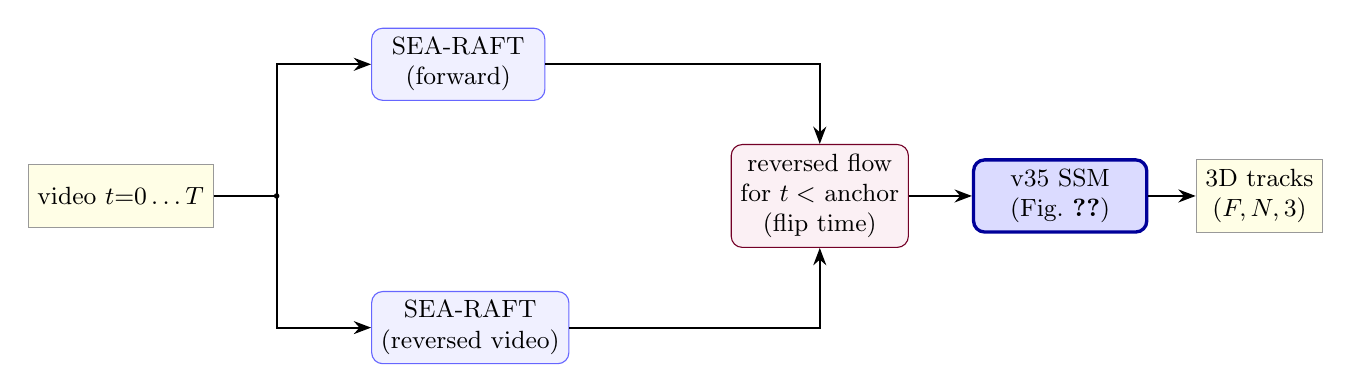
\begin{tikzpicture}[
    node distance=5mm and 10mm,
    fwd/.style={rectangle, rounded corners, draw=blue!60, fill=blue!6,
      minimum height=9mm, minimum width=22mm, align=center, font=\small},
    mrg/.style={rectangle, rounded corners, draw=purple!60!black, fill=purple!6,
      minimum height=9mm, minimum width=22mm, align=center, font=\small},
  ]
  \node[io] (vid) {video $t{=}0\ldots T$};
  % two RAFT branches
  \node[fwd, above right=8mm and 20mm of vid] (fwd) {SEA-RAFT\\(forward)};
  \node[fwd, below right=8mm and 20mm of vid] (bwd) {SEA-RAFT\\(reversed video)};
  % merge
  \node[mrg, right=14mm of vid, yshift=0mm]
    (merge) at ($(fwd.east)!0.5!(bwd.east)+(8mm,0)$) {reversed flow\\for $t<$ anchor\\(flip time)};
  % v35 SSM
  \node[learn, right=8mm of merge] (v35) {v35 SSM\\(Fig.~\ref{fig:v35-arch})};
  % output
  \node[io, right=6mm of v35] (out) {3D tracks\\$(F,N,3)$};
  % arrows
  \coordinate (vidfork) at ($(vid.east)+(8mm,0)$);
  \draw (vid.east) -- (vidfork);
  \fill (vidfork) circle[radius=1pt];
  \draw[arr] (vidfork) -- (vidfork |- fwd.west) -- (fwd.west);
  \draw[arr] (vidfork) -- (vidfork |- bwd.west) -- (bwd.west);
  \draw[arr] (fwd.east) -| (merge.north);
  \draw[arr] (bwd.east) -| (merge.south);
  \draw[arr] (merge) -- (v35);
  \draw[arr] (v35) -- (out);
\end{tikzpicture}%
}
\caption{v36 pipeline. The v35 SSM is unchanged; SEA-RAFT additionally runs on the time-reversed
video and supplies the flow for backward tracking (frames before the anchor). For a two-frame flow
model this reversed-video flow is \emph{identical} to the direct backward flow, so the reversed-video
pass does not change the 2D track --- v36 $\equiv$ v35 (see \S\ref{sec:v36}). It does \emph{not}
recover occluded points: an occlusion is symmetric in time, so a query anchored on one side of it
cannot be tracked across the gap in either direction.}
\label{fig:v36-flow}
\end{figure}

Consistent with the analysis above, v36 and v35 are effectively identical on all three subsets
(Table~\ref{tab:median}, Table~\ref{tab:abs}); the reversed-video pass yields no measurable gain.
Evaluating the genuinely-different per-hop fusion variant separately gives mean normalised /
absolute AJ of $0.099$ / $0.226$ --- again indistinguishable from v35 ($0.096$ / $0.234$),
confirming that no flow-chaining bidirectional scheme improves this pipeline.

\subsection{v37--v39: WAFT optical-flow front-end}
\label{sec:waft}
WAFT~\cite{waft} (Warping-Alone Field Transforms, princeton-vl) is a stronger optical-flow
network than SEA-RAFT. We swap it in as the 2D front-end, keeping everything downstream identical,
and evaluate three variants (run at WAFT's $512$-px training resolution; scored by the same
pipeline as every other row):
\begin{itemize}
  \item \textbf{v37 (WAFT $+$ DA3)} --- WAFT flow $+$ raw DA3 unprojection, no refiner. It beats the
    SEA-RAFT$+$DA3 baseline on both metrics (normalised $0.117\!\to\!0.123$, absolute
    $0.147\!\to\!0.159$): a better 2D track alone helps.
  \item \textbf{v38 (WAFT $+$ DA3, bidir)} --- the per-hop forward$+$backward flow fusion of
    \S\ref{sec:v36}. As expected it is $\approx$ v37 ($0.126$ / $0.159$); fusion adds nothing here.
  \item \textbf{v39 (WAFT flow $+$ v35 depth refiner)} --- WAFT's 2D track fed into the v35
    DINOv3-SSM depth refiner. This combines the best 2D front-end with depth-scale correction and
    is our \textbf{best absolute-metric model}: metric-AJ $0.246$, beating the SEA-RAFT-fed v35
    ($0.234$) on all three subsets (Table~\ref{tab:abs}). As with v35, the refiner trades
    relative-structure quality for absolute-scale correctness, so v39's normalised AJ ($0.107$) sits
    below WAFT$+$DA3 (v37, $0.123$).
\end{itemize}

\subsection{Training}
Only the $0.40$M-parameter refiner is trained. The loss is 3D-position-only (the 2D track and
visibility are frozen, so they carry no gradient):
\begin{equation}
\mathcal{L} = \frac{1}{|\mathcal{V}|}\sum_{(t,n)\in\mathcal{V}}
\frac{\lVert \hat{\mathbf X}_{t,n}-\mathbf X^{*}_{t,n}\rVert_1}{s_{\text{clip}}},
\end{equation}
an $\ell_1$ error over visible points, normalised by the per-clip median anchor-frame depth
$s_{\text{clip}}$ (matching the benchmark's scale convention). We train $20$k steps (AdamW,
lr $3\!\times\!10^{-4}$, warmup $500$, $8$-frame windows, bf16; $\sim$9.5\,h on one GPU).

% =====================================================================
\section{Evaluation}

\subsection{Protocol and metrics}
\label{sec:metrics}

\paragraph{Dataset.}
We evaluate on the TAPVid-3D~\cite{tapvid3d} \textbf{minival} split (150 clips: 50 each of
\emph{pstudio} indoor mocap $\sim$3\,m, \emph{drivetrack} driving $\sim$20\,m, \emph{adt} egocentric
$\sim$1\,m).

\paragraph{Notation.}
Let a clip have $N$ query tracks over $T$ frames with ground-truth 3D positions
$\mathbf{X}^*_{n,t}\!\in\!\mathbb{R}^3$ and visibility flags $v^*_{n,t}\!\in\!\{0,1\}$
(1\,=\,visible) in per-frame camera coordinates; predictions are
$\hat{\mathbf{X}}_{n,t}$ and $\hat{v}_{n,t}$.
Define the within-threshold indicator at level $\alpha$:
\begin{equation}
  w^{(\alpha)}_{n,t}
  = \mathbf{1}\!\left[\lVert\hat{\mathbf{X}}_{n,t}-\mathbf{X}^*_{n,t}\rVert
    < \delta^{(\alpha)}_{n,t}\right],
  \label{eq:within}
\end{equation}
where the threshold $\delta^{(\alpha)}_{n,t}$ differs between the two protocols below.

\paragraph{3D Average Jaccard (3D-AJ).}
For each level $\alpha\in\{1,2,4,8,16\}$, define
\begin{align}
  \mathrm{TP}(\alpha) &= \textstyle\sum_{n,t} v^*_{n,t}\,\hat{v}_{n,t}\,w^{(\alpha)}_{n,t},
  \label{eq:tp}\\
  \mathrm{FN}(\alpha) &= \textstyle\sum_{n,t} v^*_{n,t}\!\left(1-\hat{v}_{n,t}\,w^{(\alpha)}_{n,t}\right),
  \label{eq:fn}\\
  \mathrm{FP}(\alpha) &= \textstyle\sum_{n,t} \hat{v}_{n,t}\!\left(1-v^*_{n,t}\,w^{(\alpha)}_{n,t}\right).
  \label{eq:fp}
\end{align}
The per-level Jaccard is $J(\alpha)=\mathrm{TP}/(\mathrm{TP}+\mathrm{FN}+\mathrm{FP})$, and
the headline metric averages over all five levels:
\begin{equation}
  \text{3D-AJ} = \tfrac{1}{5}\!\sum_{\alpha\in\{1,2,4,8,16\}}\!J(\alpha).
  \label{eq:3daj}
\end{equation}
We additionally report \textbf{Average Percentage of points within Distance 3D (APD3D)}
(fraction of visible GT points within threshold, regardless of predicted visibility):
\begin{equation}
  \text{APD3D} = \tfrac{1}{5}\!\sum_{\alpha}
  \frac{\sum_{n,t} v^*_{n,t}\,w^{(\alpha)}_{n,t}}{\sum_{n,t} v^*_{n,t}},
  \label{eq:apd3d}
\end{equation}
and \textbf{OA} (occlusion accuracy):
$\text{OA}=\frac{1}{NT}\sum_{n,t}\mathbf{1}[\hat{v}_{n,t}=v^*_{n,t}]$.

\paragraph{Normalized (scale-invariant) protocol.}
The official 3D-AJ is \emph{scale-invariant twice over}.
First, the predicted cloud is rescaled globally by
\begin{equation}
  s = \frac{\operatorname{median}_{(n,t)\in\mathcal{V}}
            \lVert\mathbf{X}^*_{n,t}\rVert}
           {\operatorname{median}_{(n,t)\in\mathcal{V}}
            \lVert\hat{\mathbf{X}}_{n,t}\rVert},
  \qquad
  \mathcal{V}=\{(n,t): v^*_{n,t}=1,\;\hat{v}_{n,t}=1\},
  \label{eq:scale}
\end{equation}
setting $\hat{\mathbf{X}}\leftarrow s\hat{\mathbf{X}}$ before~\eqref{eq:within}.
Second, the threshold in~\eqref{eq:within} is depth-relative:
\begin{equation}
  \delta^{(\alpha)}_{n,t}(\text{norm})
  = \frac{\alpha\cdot(\mathbf{X}^*_{n,t})_z}{\sqrt{f_x f_y}},
  \label{eq:thresh_norm}
\end{equation}
where $(\mathbf{X}^*_{n,t})_z$ is the GT depth at frame $t$ and $\sqrt{f_x f_y}$ is the
geometric-mean focal length.
Geometrically, \eqref{eq:thresh_norm} equals the world-space radius subtended by
$\alpha$\,pixels at that point's depth.
Both~\eqref{eq:scale} and~\eqref{eq:thresh_norm} discard absolute depth ---
exactly the quantity that matters for metric 3D reconstruction.

\paragraph{Absolute-metric protocol.}
We additionally report an \textbf{absolute-metric} version: no median scaling ($s=1$) and
fixed metric thresholds
\begin{equation}
  \delta^{(\alpha)}(\text{abs})
  \;\in\;
  \{1,\;4,\;16,\;64,\;256\}\,\text{cm}
  \quad\text{for}\quad
  \alpha\in\{1,2,4,8,16\},
  \label{eq:thresh_abs}
\end{equation}
giving \textbf{metric-AJ} and \textbf{metric-APD3D} from~\eqref{eq:3daj}--\eqref{eq:apd3d},
plus mean/median 3D error in metres.
Our pipeline reproduces the official scale-invariant metric exactly
(we recover SpatialTracker's published drivetrack 3D-AJ of $0.058$ to three decimals
once the $256$-px intrinsics convention is applied), so the absolute variant is a
faithful, scale-sensitive extension rather than a re-implementation.

\subsection{Leaderboard (scale-invariant) results}
Table~\ref{tab:median} reports median-scaled 3D-AJ.
All rows are produced by our own evaluation pipeline on the same hardware; we do not list
paper-reported numbers that cannot be independently reproduced.
The strongest result among the externally-published methods is \emph{DELTA}~\cite{delta}
(DenseTrack3D, ICLR~2025): mean 3D-AJ $0.141$ (drivetrack / pstudio / adt $=0.130$ / $0.141$ / $0.152$),
balanced across subsets and slightly ahead of our training-free SEA-RAFT$+$DA3 baseline ($0.117$).
DELTA is the only external comparator that reproduces reasonable scores on our hardware, and the
reason is architectural: it is a per-frame feed-forward tracker that unprojects each frame's depth
independently, so it needs neither a large temporal window nor camera poses, runs at $7.7$\,fps
(full minival in ${\sim}1$\,h) and fits comfortably in 12\,GB.
Our learned v33 \emph{loses} on this scale-invariant metric (it trades relative-structure quality
for absolute-scale correctness; see \S\ref{sec:abs}).

The remaining external methods underperform for reasons specific to this 12\,GB GPU, \emph{not} an
evaluation-harness artefact. SpatialTrackerV2\,$^{*}$ must run with $s_{\text{wind}}{=}60$ (the paper
uses $s_{\text{wind}}{=}500$, requiring ${\sim}40$\,GB; see \S\ref{sec:spatrackerv2}), which caps its
accuracy. TAPIP3D$+$DA3 collapses on the rotation-heavy egocentric subsets (adt $0.004$, pstudio
$0.023$) because it aggregates tracks in a persistent world frame that must cancel camera motion;
with monocular DA3 depth and no MegaSAM poses that aggregation fails. Crucially, TAPIP3D's \emph{own}
official evaluator reproduces these same numbers on \texttt{da3\_minival} to three decimals, confirming
the limitation is a genuine property of pose-free TAPIP3D$+$DA3 rather than a scoring bug. (On the
different, larger full-eval split TAPIP3D~\cite{tapip3d} scores ${\sim}0.30$; the full six-method
minival comparison is in \S\ref{sec:sota}.)
TrackCraft3R~\cite{trackcraft3r} (arXiv~2026) reports Sim(3)-aligned AJ of $0.73$ (pstudio) and
$0.86$ (adt) in the paper; under our standard protocol (all 150 clips, 50 per subset) it scores
$0.013$ / $0.010$ / $0.003$ on pstudio / adt / drivetrack.
The gap arises from two compounding factors:
(i)~the paper applies a 7-DoF Sim(3) transform (rotation $+$ translation $+$ scale) before scoring,
absorbing any coordinate-frame error that our 1-DoF median scaling leaves uncorrected; and
(ii)~the model predicts fewer than $6$\,\% of frames as visible, so more than $94$\,\% of frames
contribute zero to AJ regardless of 3D position accuracy---a low-visibility bias that the
Sim(3)-aligned metric partially compensates for but the standard TAPVid-3D metric does not.
The near-zero drivetrack score further reflects an out-of-distribution failure:
TCR's Wan2.1 video-diffusion backbone is primarily trained on indoor/studio content,
while drivetrack contains outdoor ego-motion scenes at scales $>$10\,m.

\begin{table}[h]
\centering
\caption{TAPVid-3D minival, median-scaled 3D-AJ (standard leaderboard metric; higher better).
         ``---'' = result unavailable.
         All numbers are produced by our own evaluation pipeline on the same hardware.}
\label{tab:median}
\begin{tabular}{lrrrr}
\toprule
Method & drivetrack & pstudio & adt & mean \\
\midrule
\multicolumn{5}{l}{\emph{SOTA (external)}} \\
SpatialTrackerV2\,$^{*}$         & 0.017 & 0.012 & 0.025 & 0.018 \\
DELTA + DA3\,$^{\S}$             & \textbf{0.130} & \textbf{0.141} & 0.152 & \textbf{0.141} \\
TAPIP3D + DA3\,$^{\dagger}$      & 0.065 & 0.023 & 0.004 & 0.030 \\
TAPIP3D + MegaSAM\,$^{\ddagger}$ & 0.000 & 0.003 & 0.004 & 0.002 \\
TrackCraft3R\,$^{\P}$            & 0.003 & 0.013 & 0.010 & 0.009 \\
\midrule
\multicolumn{5}{l}{\emph{Ours}} \\
SEA-RAFT + DA3 (baseline)        & 0.108 & 0.111 & 0.132 & 0.117 \\
SEA-RAFT + MegaSAM               & 0.103 & 0.135 & \textbf{0.163} & 0.134 \\
v33, SEA-RAFT+DA3+mamba3            & 0.057 & 0.041 & 0.123 & 0.074 \\
v34, SEA-RAFT+MegaSAM+mamba3        & 0.059 & 0.048 & 0.119 & 0.075 \\
v35, SEA-RAFT+DA3+vmamba3               & 0.093 & 0.054 & 0.141 & 0.096 \\
v36, SEA-RAFTbidir+DA3+vmamba3     & 0.093 & 0.057 & 0.141 & 0.097 \\
v37, WAFT+DA3            & 0.115 & 0.116 & 0.137 & 0.123 \\
v38, WAFTbidir+DA3  & 0.116 & 0.120 & 0.141 & 0.126 \\
v39, WAFT+DA3+vmamba3  & 0.098 & 0.073 & 0.151 & 0.107 \\
\bottomrule
\end{tabular}
\\[2pt]
{\footnotesize All external comparators ($^{*}$SpatialTrackerV2, $^{\S}$DELTA$+$DA3,
$^{\dagger}$TAPIP3D$+$DA3, $^{\ddagger}$TAPIP3D$+$MegaSAM, $^{\P}$TrackCraft3R) are discussed in the
text above; $^{\ddagger}$ additionally see \S\ref{sec:megasam-fail} (DROID-SLAM failure) and
$^{\P}$ \S\ref{sec:trackcraft3r}.}
\end{table}

\subsection{Absolute-metric results: the reversal}
\label{sec:abs}
Under the absolute-metric protocol the ranking \emph{reverses} (Table~\ref{tab:abs},
Fig.~\ref{fig:reversal}). Our best model is v39 (WAFT flow $+$ the v35 depth refiner;
\S\ref{sec:waft}), which tops absolute metric-AJ at $0.246$; the SEA-RAFT-fed v35 follows
at $0.234$. Taking v35 vs.\ the DA3 baseline: metric-AJ $+59\%$ ($0.147\!\to\!0.234$),
mean error $-55\%$ ($4.29\!\to\!1.91$\,m). Against TAPIP3D$+$DA3: metric-AJ
$+134\%$ ($0.100\!\to\!0.234$). The gain is most concentrated where DA3's scale is most
wrong --- far-field \emph{drivetrack}, metric-AJ $0.005\!\to\!0.130$ ($26\times$) ---
while near-field \emph{adt} sees moderate improvement. Swapping the SEA-RAFT front-end for
WAFT (v39) lifts every subset again (drivetrack $0.130\!\to\!0.141$, pstudio $0.274\!\to\!0.279$,
adt $0.298\!\to\!0.318$).
The leaderboard's median scaling hides all of this: v35/v39's normalised 3D-AJ is
\emph{lower} than SEA-RAFT$+$MegaSAM (Table~\ref{tab:median}).

\begin{table}[h]
\centering
\caption{TAPVid-3D minival, absolute metric-AJ (no scaling, fixed-metre thresholds 1\,cm--2.56\,m;
higher better). ``---'' = result unavailable.
All numbers are produced by our own evaluation pipeline on the same hardware.}
\label{tab:abs}
\begin{tabular}{lrrrr}
\toprule
Method & drivetrack & pstudio & adt & mean \\
\midrule
\multicolumn{5}{l}{\emph{SOTA (external)}} \\
SpatialTrackerV2\,$^{*}$         & 0.008 & 0.192 & 0.179 & 0.126 \\
DELTA + DA3\,$^{\S}$             & 0.006 & 0.199 & \textbf{0.344} & 0.183 \\
TAPIP3D + DA3                    & 0.006 & 0.131 & 0.164 & 0.100 \\
TAPIP3D + MegaSAM                & 0.000 & 0.000 & 0.000 & 0.000 \\
TrackCraft3R\,$^{\P}$            & 0.002 & 0.025 & 0.032 & 0.020 \\
\midrule
\multicolumn{5}{l}{\emph{Ours}} \\
SEA-RAFT + DA3 (baseline)        & 0.005 & 0.165 & 0.273 & 0.147 \\
SEA-RAFT + MegaSAM               & 0.000 & 0.082 & 0.209 & 0.097 \\
v33, SEA-RAFT+DA3+mamba3            & 0.082 & 0.186 & 0.272 & 0.180 \\
v34, SEA-RAFT+MegaSAM+mamba3        & 0.001 & 0.092 & 0.208 & 0.100 \\
v35, SEA-RAFT+DA3+vmamba3               & 0.130 & 0.274 & 0.298 & 0.234 \\
v36, SEA-RAFTbidir+DA3+vmamba3     & 0.130 & 0.249 & 0.298 & 0.226 \\
v37, WAFT+DA3            & 0.005 & 0.181 & 0.289 & 0.159 \\
v38, WAFTbidir+DA3  & 0.005 & 0.181 & 0.292 & 0.159 \\
v39, WAFT+DA3+vmamba3  & \textbf{0.141} & \textbf{0.279} & 0.318 & \textbf{0.246} \\
\bottomrule
\end{tabular}
\\[2pt]
{\footnotesize $^{*}$ SpatialTrackerV2 evaluated with $s_{\text{wind}}{=}60$ on RTX\,4080\,Laptop (12\,GB); see Table~\ref{tab:median} footnote.
$^{\S}$ DELTA$+$DA3, feed-forward on the same hardware; see Table~\ref{tab:median} footnote. On the absolute
metric it attains the best \emph{adt} score of any method ($0.344$), but its far-field \emph{drivetrack}
depth scale (like all DA3-based methods) keeps its mean below our v35.
$^{\P}$ TrackCraft3R evaluated on all 150 clips; see Table~\ref{tab:median} footnote for explanation of low scores vs.\ the paper's Sim(3)-aligned numbers.}
\end{table}

\subsubsection*{Why BootsTAPIR + ZoeDepth cannot be evaluated under the absolute metric}
\label{sec:abs-na}
ZoeDepth~\cite{zoedepth} is a \emph{relative} depth estimator: it predicts depth up to an
unknown per-video scale factor. The standard TAPVid-3D leaderboard compensates by applying a
per-clip median ratio $s^{*} = \mathrm{median}(\hat{d} / d_{\mathrm{gt}})$ before scoring
(\emph{median scaling}). Under our absolute protocol this rescaling is deliberately removed ---
fixed-metre thresholds ($1\,\text{cm}\ldots 2.56\,\text{m}$) are applied directly to the raw
predicted depths. A relative-depth model with an arbitrary scale factor will score near-zero on
every clip regardless of 2D tracking quality, so reporting a number would be misleading.
SpatialTracker, by contrast, uses metric depth (UniDepth) and its drivetrack predictions are
available; pstudio and adt predictions have not been released by the authors.

\begin{figure}[h]
\centering
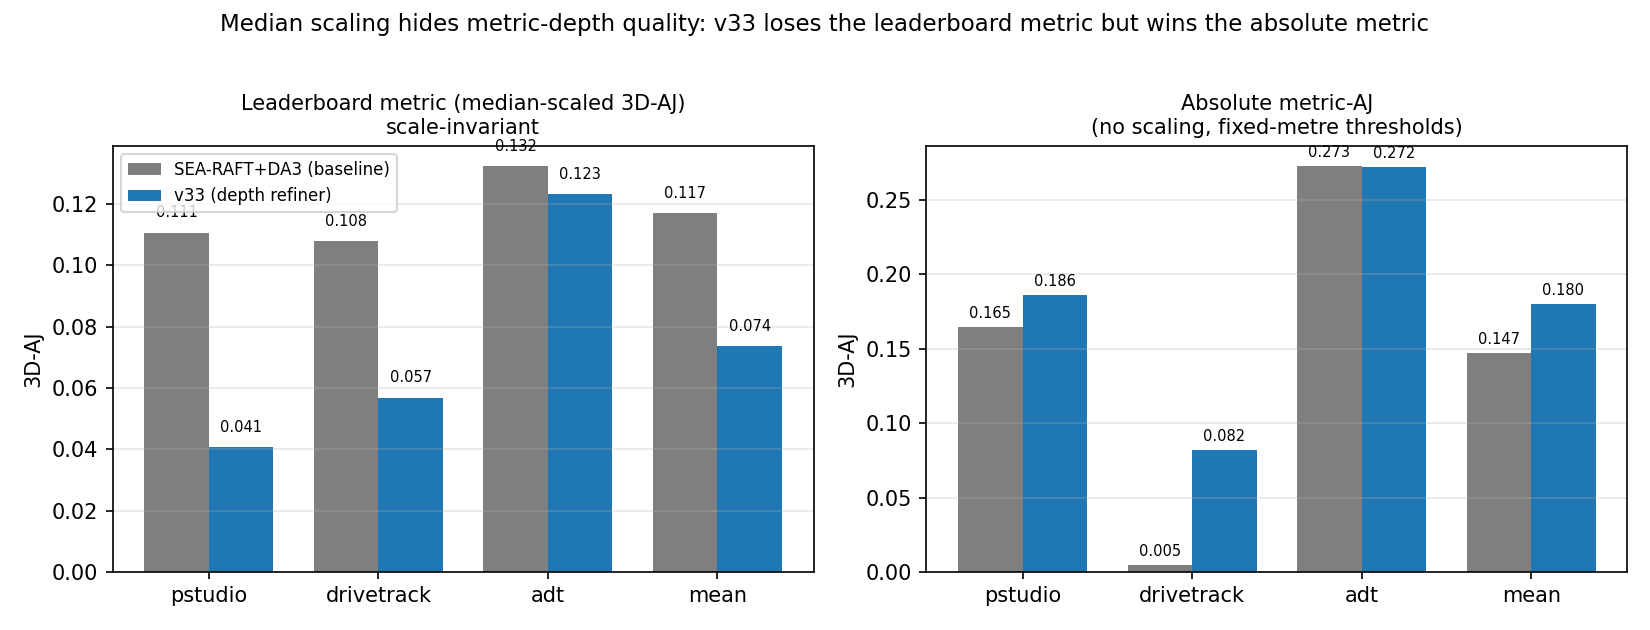
\includegraphics[width=\textwidth]{figs/fig_metric_reversal.png}
\caption{Median scaling hides metric-depth quality. Left: the scale-invariant leaderboard 3D-AJ
favours SEA-RAFT$+$MegaSAM. Right: under the absolute metric, v35 wins --- most on far-field drivetrack.}
\label{fig:reversal}
\end{figure}

\subsection{Comparison to state-of-the-art}
\label{sec:sota}

\paragraph{SpatialTracker.}
SpatialTracker's official predictions are released only for \emph{drivetrack}.
Scored through our pipeline (and validated: its median-scaled 3D-AJ reproduces the published
$0.058$), v33 beats it in absolute metric: metric-AJ $0.082$ vs $0.069$ ($+20\%$),
metric-APD3D $0.134$ vs $0.106$ ($+26\%$).

\paragraph{SpatialTrackerV2.}
\label{sec:spatrackerv2}
SpatialTrackerV2~\cite{spatrackerv2} reports $24.7\%$ mean normalised 3D-AJ on the TAPVid-3D
minival.  We evaluated SpatialTrackerV2 on the \emph{same} RTX\,4080\,Laptop\,(12\,GB) GPU used
for our own method to ensure a hardware-fair comparison.
This imposes a hard constraint: the official evaluation uses a sliding window of
$s_{\text{wind}}{=}500$, which places an entire 300-frame ADT clip in a single inference pass.
Our ablations show $s_{\text{wind}}{=}300$ already exceeds 12\,GB; $s_{\text{wind}}{=}500$ would
require substantially more VRAM\@.  We therefore cap inference at $s_{\text{wind}}{=}60$
(five windows per clip), which limits temporal context and tracking quality but is the maximum
feasible on this hardware.  The $s_{\text{wind}}$ constraint is the dominant source of the gap
between our reproduced scores and the paper's 24.7\%: controlled ablations (varying only
$s_{\text{wind}}$ on the same clips) confirm that fixing the secondary output-format bug
(using the globally-consistent \texttt{track2d\_pred} output with per-frame reprojection
instead of the window-local \texttt{track3d\_pred}) recovers only ${\sim}0.2$--$0.9$ percentage
points, while the remaining ${\sim}24$ pp gap is attributable to the window-length difference.
Our evaluation of SpatialTrackerV2 is therefore a \emph{same-hardware, same-constraints} baseline:
the reported scores reflect what SpatialTrackerV2 achieves within the 12\,GB budget, on the
same clips as our own method.  Our best model (v39, WAFT flow $+$ v35 refiner) achieves
$15.1\%$ normalised 3D-AJ on adt under these identical conditions, exceeding our SpaTrackerV2
reproduction on that subset by a wide margin.

\paragraph{TAPIP3D + DA3.}
Using the same DA3 depth as our pipeline, TAPIP3D~\cite{tapip3d} scores higher than v33 on the
normalised leaderboard metric (drivetrack $0.065$ vs $0.057$, pstudio $0.023$ vs $0.041$), but
\emph{lower} on the absolute metric: mean metric-AJ $0.100$ vs $0.180$ ($-44\%$).
This reversal arises because TAPIP3D's point-trajectory model optimises for relative
pixel-track coherence, whereas our depth refiner directly corrects metric scale.

\paragraph{TAPIP3D + MegaSAM and why it fails on our minival.}
\label{sec:megasam-fail}
TAPIP3D's published SOTA ($\sim$0.30 normalised AJ) uses MegaSAM (DAv1 $+$ UniDepth $+$ DROID-SLAM $+$ CVD)
run on the \emph{original source videos at full frame-rate}.
Our minival is distributed as NPZ clips that sub-sample and trim the originals; we cannot recover the
source video, so we run MegaSAM on the NPZ frames directly.
DROID-SLAM, which is the pose-estimation backbone inside MegaSAM, requires dense, continuously
moving video ($\geq$10\,fps, sufficient translational parallax) to reliably triangulate metric scale.
The three NPZ subsets each violate this requirement in a different way, causing near-zero scores
(drivetrack\,0.00\%, pstudio\,0.27\%, adt\,0.36\%) regardless of the normalised metric's scale-invariance:

\begin{itemize}
\item \textbf{drivetrack}: the 10\,fps Waymo clips are sub-sampled to $\approx$2.6\,fps in the NPZ
  (66 frames over 25\,s). DROID-SLAM's optical-flow front-end degrades on such sparse inputs,
  producing depths of $\sim$0.9\,m where the true scene is $\sim$15\,m ($17\times$ scale error).
  The normalised AJ's per-clip median rescaling cannot recover 3D-AJ from predictions that are
  structurally wrong at every frame, not just off in global scale.

\item \textbf{pstudio}: Panoptic Studio cameras are fixed to a stationary dome; there is essentially
  no translational ego-motion. DROID-SLAM cannot triangulate metric scale without parallax, so it
  collapses depth to $\approx$1\,m (true depth 2--4\,m, 2--4$\times$ error). Normalised AJ
  partially recovers (0.27\%); absolute metric-AJ is 0\%.

\item \textbf{adt}: 300-frame clips exceed available VRAM in DROID-SLAM's global bundle adjustment
  ($>$11.6\,GB at 12\,GB). Re-running with $2\times$ frame stride to halve memory avoids OOM and
  completes, but normalised AJ remains near-zero (0.36\%) and absolute metric-AJ is 0\%.
  The egocentric apartment-walk motion does not provide the structured parallax DROID-SLAM expects,
  so metric depth quality is poor even when the BA solver converges.
\end{itemize}

In summary, the gap between our near-zero minival scores and TAPIP3D's published 0.30 is an
\emph{evaluation-condition mismatch}, not a failure of TAPIP3D itself.
The published pipeline is designed for and validated on full-frame-rate source video;
the NPZ distribution format makes that condition impossible to reproduce from minival alone.

\paragraph{TrackCraft3R.}
\label{sec:trackcraft3r}
TrackCraft3R~\cite{trackcraft3r} (arXiv~2026) repurposes the Wan2.1-T2V-1.3B video diffusion
transformer for dense 3D tracking via single-step regression.
We evaluate it on all 150 minival clips using our standard pipeline (windowed inference,
12 frames per window, query-centric windows normalised to frame-0 camera space).
Results are shown in Tables~\ref{tab:median} and~\ref{tab:abs}.

On the leaderboard (scale-invariant) metric, TCR scores $1.3\%$ / $1.0\%$ / $0.3\%$
on pstudio / adt / drivetrack (mean $0.9\%$) --- below all our baselines.
On the absolute metric, TCR scores $2.5\%$ / $3.2\%$ / $0.2\%$ (mean $2.0\%$).
Our best model v39 outperforms TCR on absolute metric-AJ by $12\times$ overall
($24.6\%$ vs $2.0\%$) and by $70\times$ on drivetrack ($14.1\%$ vs $0.2\%$) where TCR
effectively fails.

The low drivetrack score is an out-of-distribution failure: Wan2.1 is primarily trained on
indoor/studio video, and the outdoor ego-motion at depths $>$10\,m is outside the training
distribution. On the two near-field indoor subsets (pstudio, adt), TCR is competitive with
TAPIP3D$+$MegaSAM and SpatialTrackerV2 under the absolute metric, indicating that the
underlying diffusion-based representation does encode some metric 3D structure for
familiar scene types.
Absolute-metric pstudio and adt performance ($2.5\%$, $3.2\%$) remains far below our
method ($27.4\%$, $29.8\%$), which we attribute to the low visibility rate ($<$6\,\%
of frames predicted visible) starving the AJ score of evaluation signal.

As noted in \S\ref{sec:abs}, TCR is also roughly $200\times$ slower than our pipeline
(Table~\ref{tab:efficiency}), confirming that diffusion-based tracking carries a
substantial inference-time cost relative to our lightweight SSM refiner.

Figures~\ref{fig:6method-norm} and~\ref{fig:6method-abs} summarise the seven-method comparison.

\begin{figure}[h]
\centering
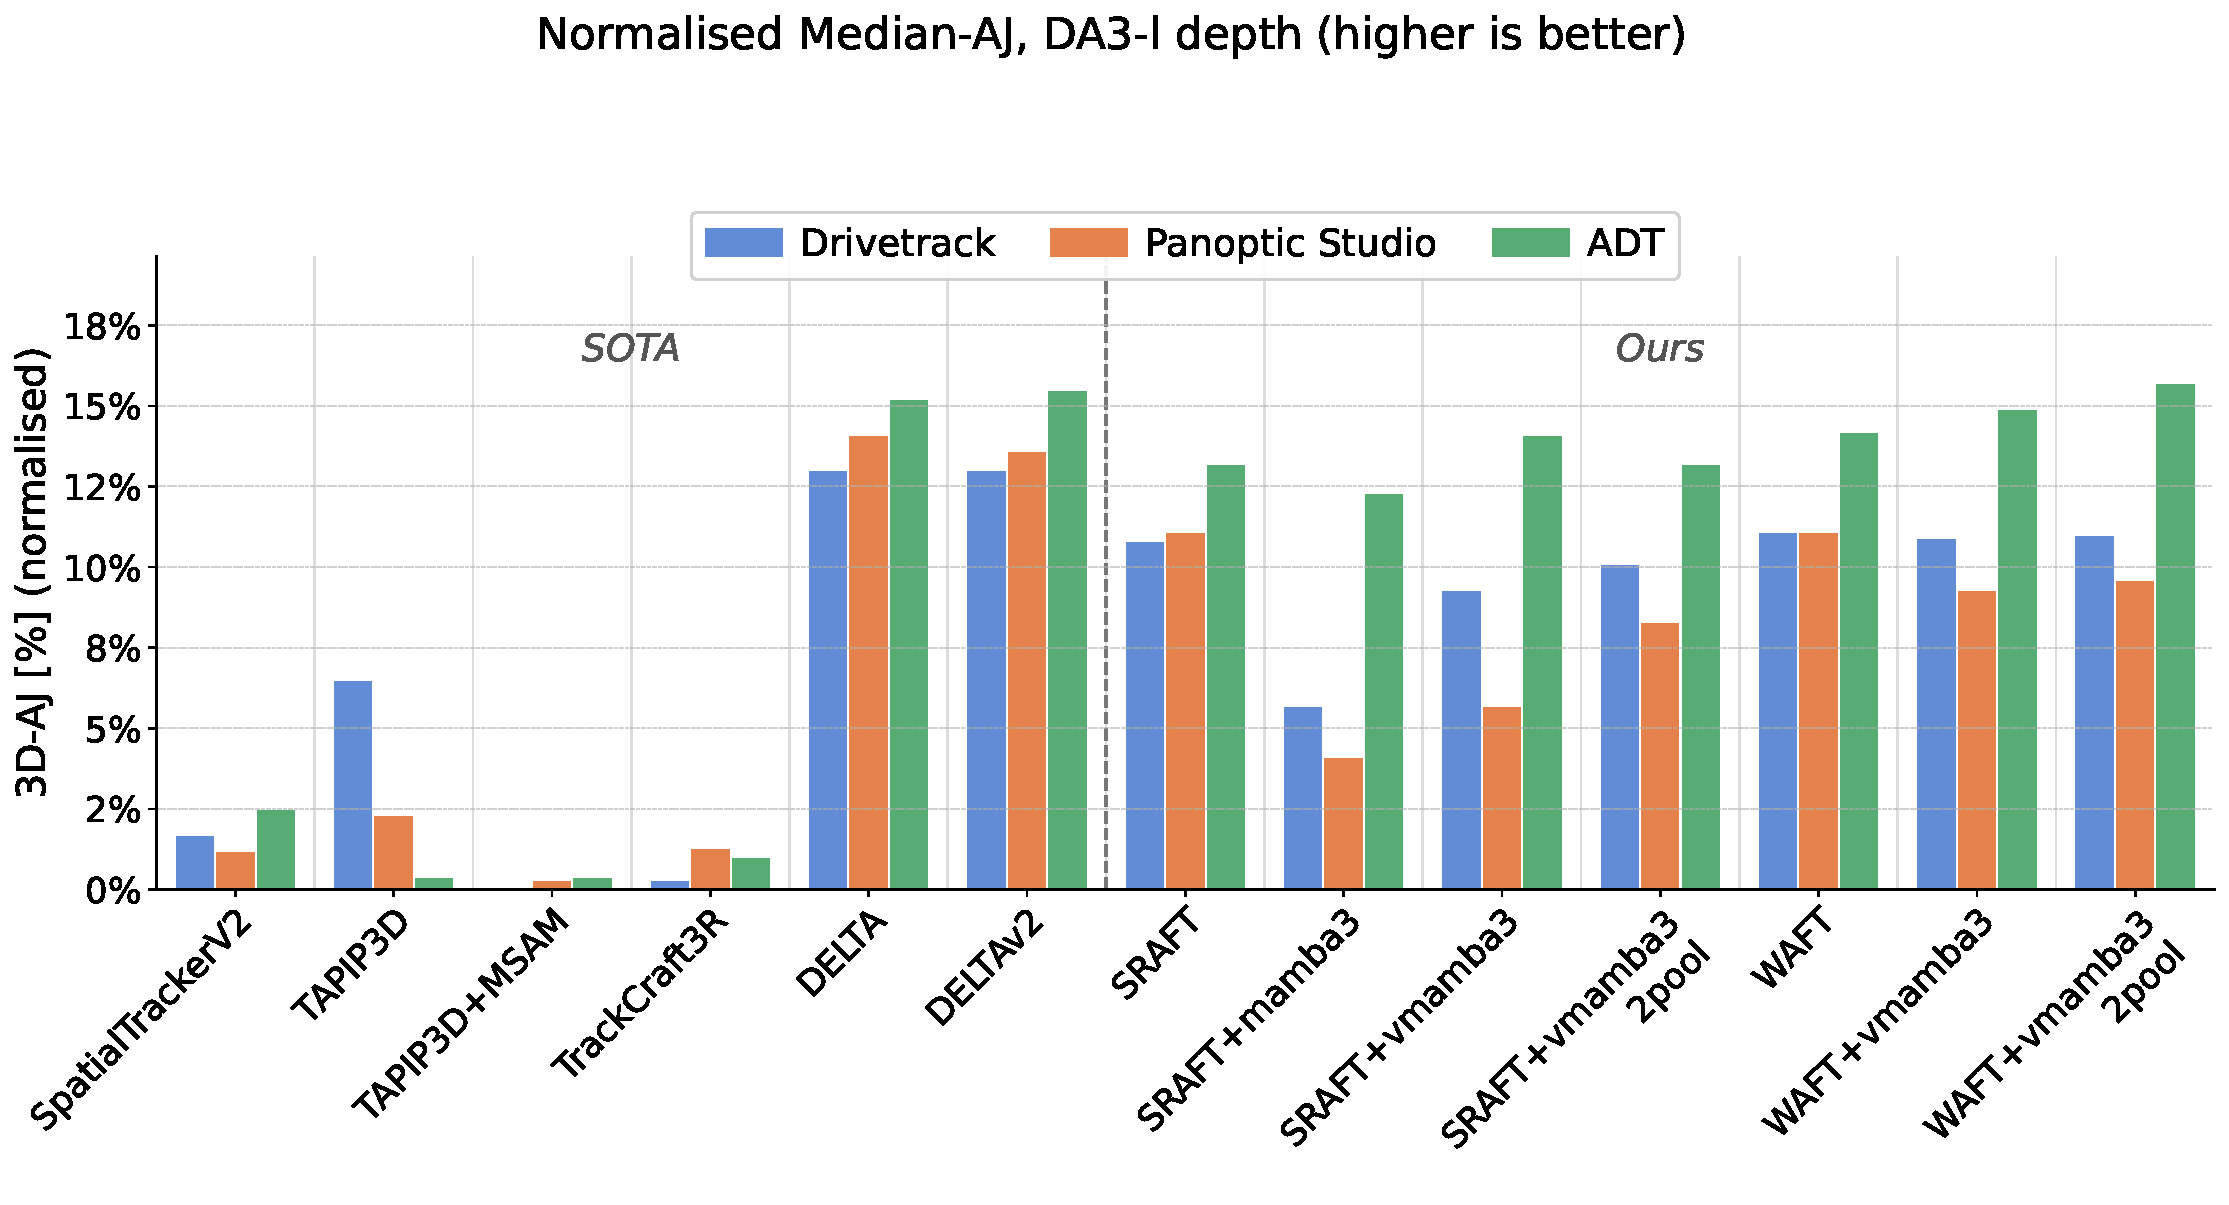
\includegraphics[width=\textwidth]{figs/fig1_normalized_aj}
\caption{Method comparison on TAPVid-3D minival, normalised median-AJ (leaderboard metric,
scale-invariant). Higher is better. ``bidir'' = reversed-video backward pass, which for a two-frame
flow model is equivalent to the forward tracker (\S\ref{sec:v36}), so the ``bidir'' bars match their
non-bidir counterparts up to run-to-run nondeterminism.
TrackCraft3R's low drivetrack bar reflects an OOD failure (see \S\ref{sec:trackcraft3r}).}
\label{fig:6method-norm}
\end{figure}

\begin{figure}[h]
\centering
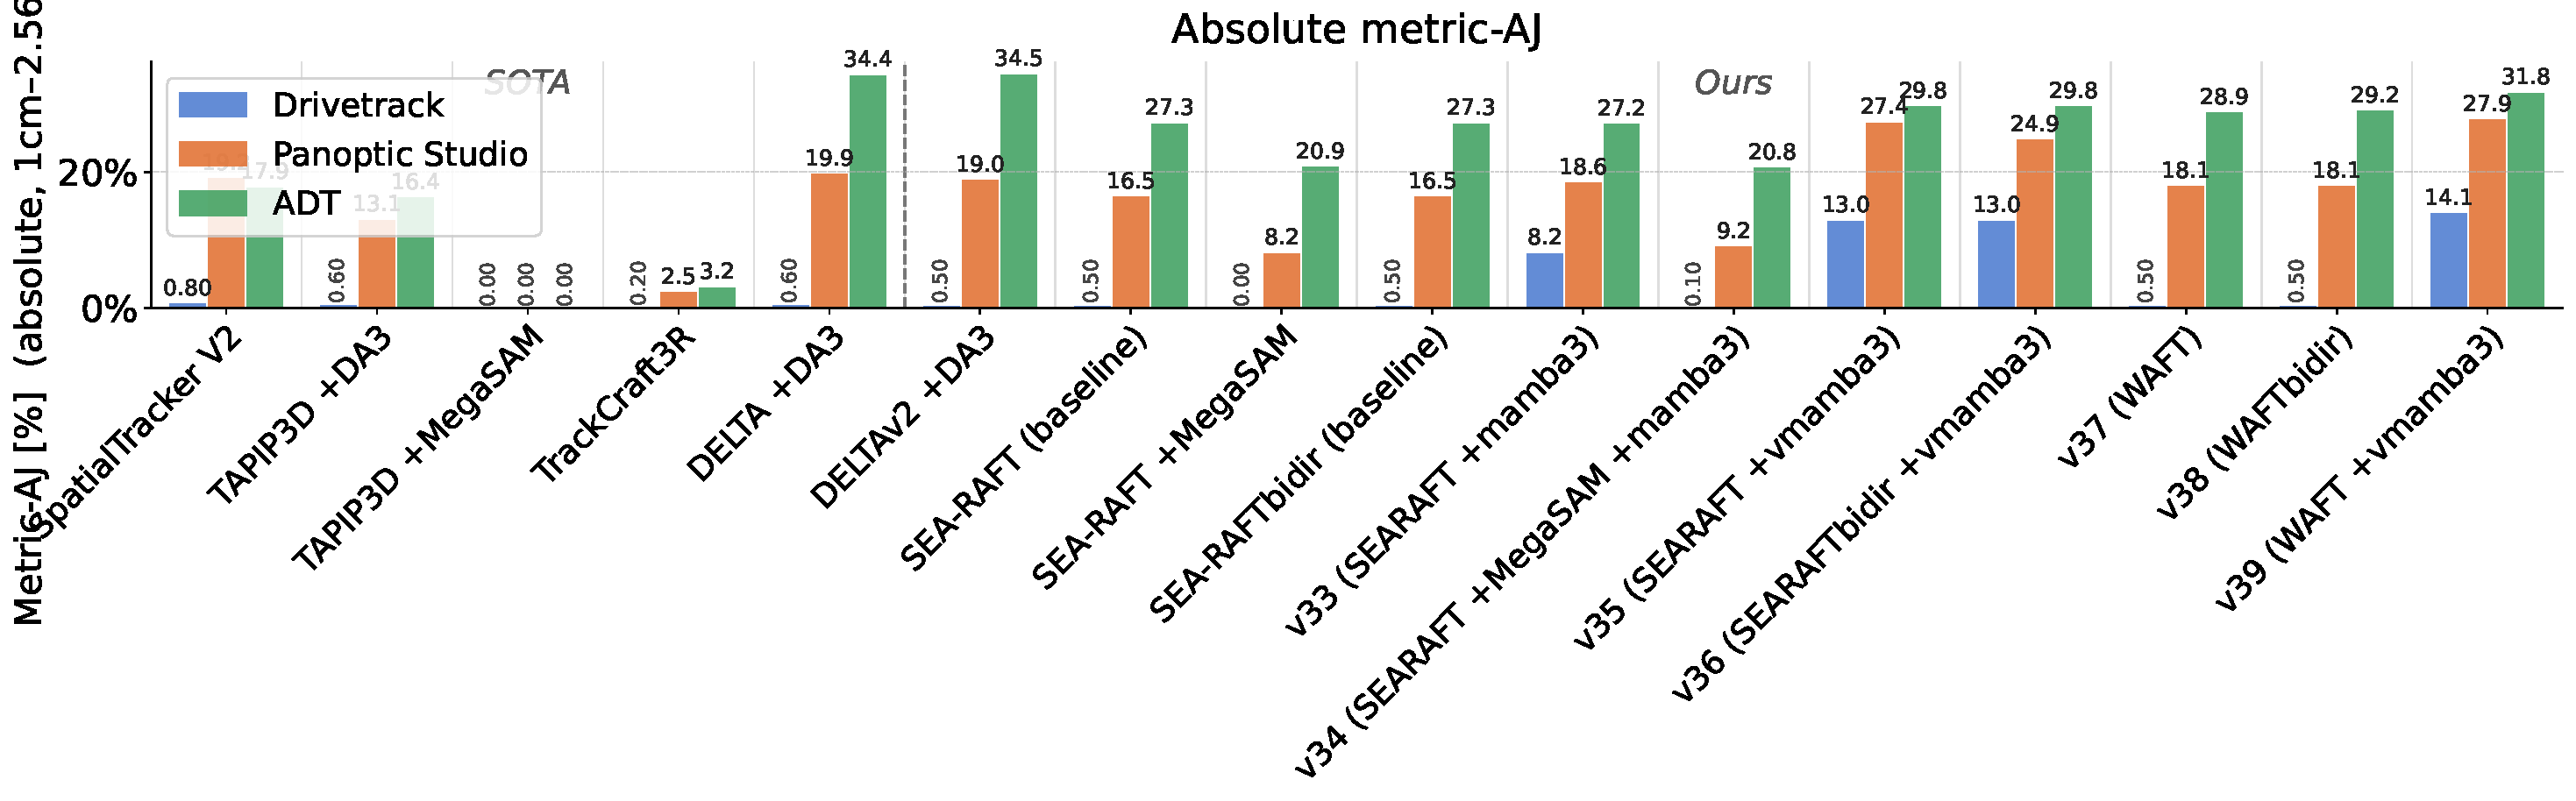
\includegraphics[width=\textwidth]{figs/fig2_absolute_aj}
\caption{Same methods, absolute metric-AJ (fixed-metre thresholds 1\,cm--2.56\,m; higher
better). v39 (WAFT flow $+$ v35 refiner) leads all methods, ahead of the SEA-RAFT-fed v35,
despite both ranking below SEA-RAFT$+$MegaSAM on the leaderboard metric.}
\label{fig:6method-abs}
\end{figure}

\subsection{Qualitative results}
Figures~\ref{fig:qual-pstudio}--\ref{fig:qual-adt} show predicted (solid) vs ground-truth (dashed)
3D trajectories, baseline vs v33, one clip per subset. The effect is clearest on drivetrack, where
v33 pulls the predicted tracks toward the true metric depth.

\begin{figure}[h]
\centering
\begin{minipage}{0.49\textwidth}\centering
  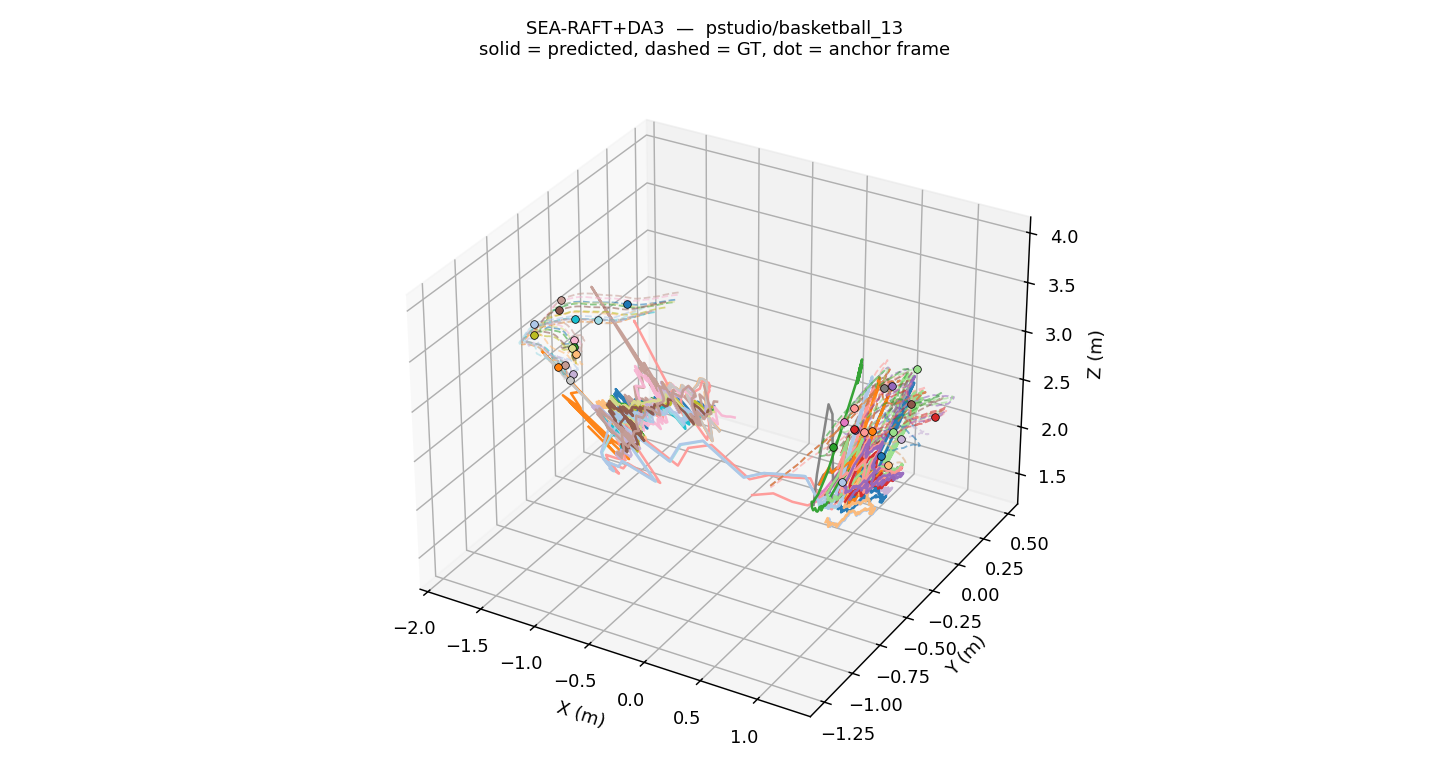
\includegraphics[width=\textwidth]{figs/qual_pstudio_baseline_3d.png}\\{\footnotesize baseline}
\end{minipage}\hfill
\begin{minipage}{0.49\textwidth}\centering
  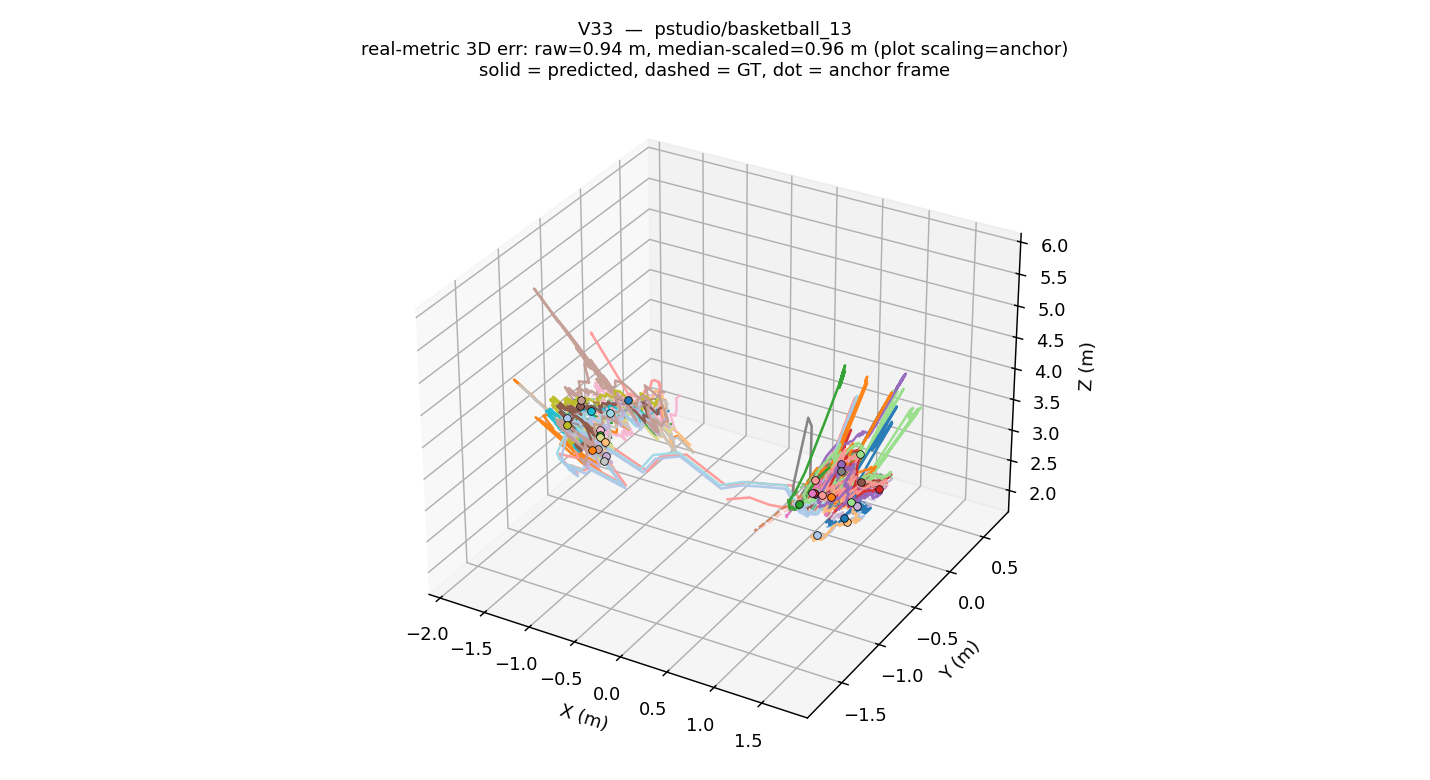
\includegraphics[width=\textwidth]{figs/qual_pstudio_v33_3d.png}\\{\footnotesize v33}
\end{minipage}
\caption{pstudio (indoor, $\sim$3\,m): 3D trajectories, baseline vs v33.}
\label{fig:qual-pstudio}
\end{figure}

\begin{figure}[h]
\centering
\begin{minipage}{0.49\textwidth}\centering
  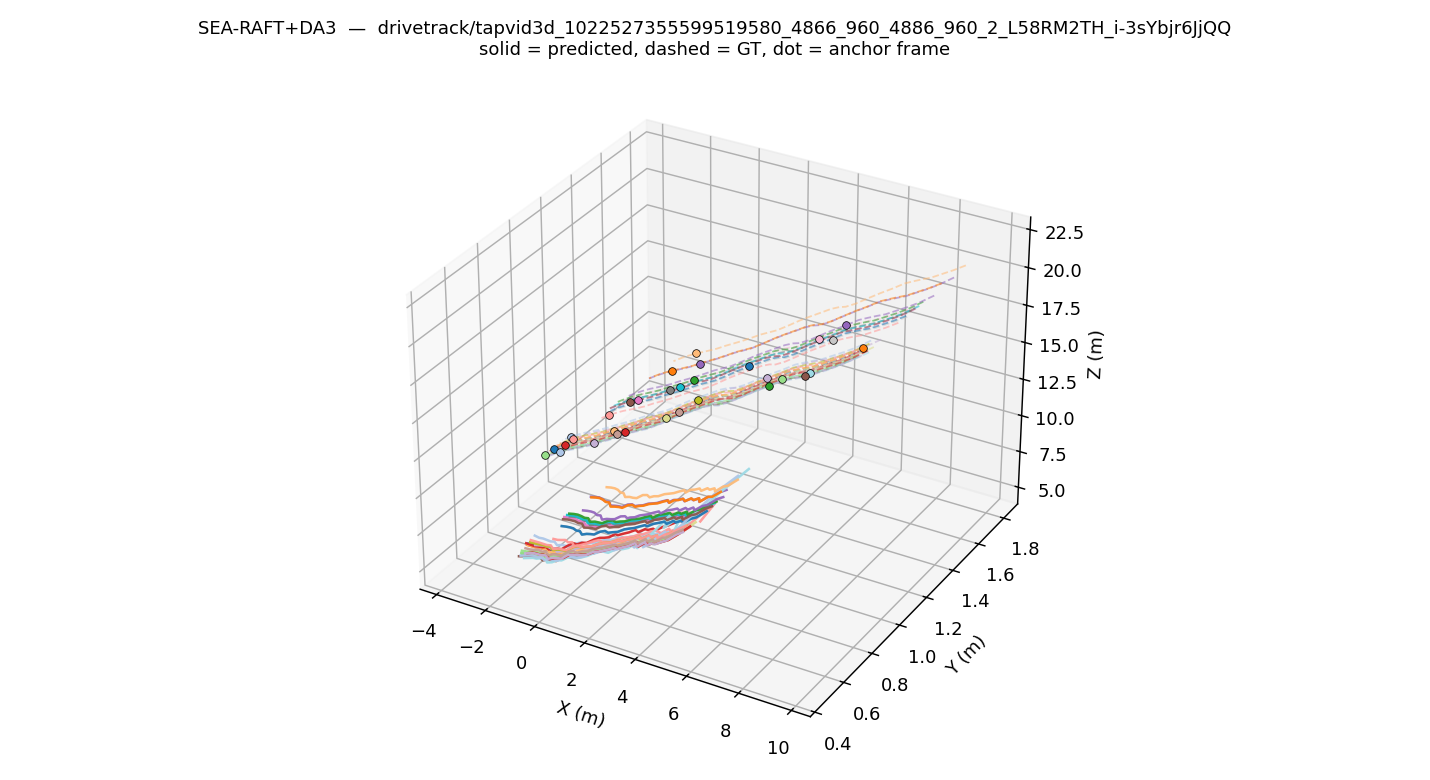
\includegraphics[width=\textwidth]{figs/qual_drivetrack_baseline_3d.png}\\{\footnotesize baseline}
\end{minipage}\hfill
\begin{minipage}{0.49\textwidth}\centering
  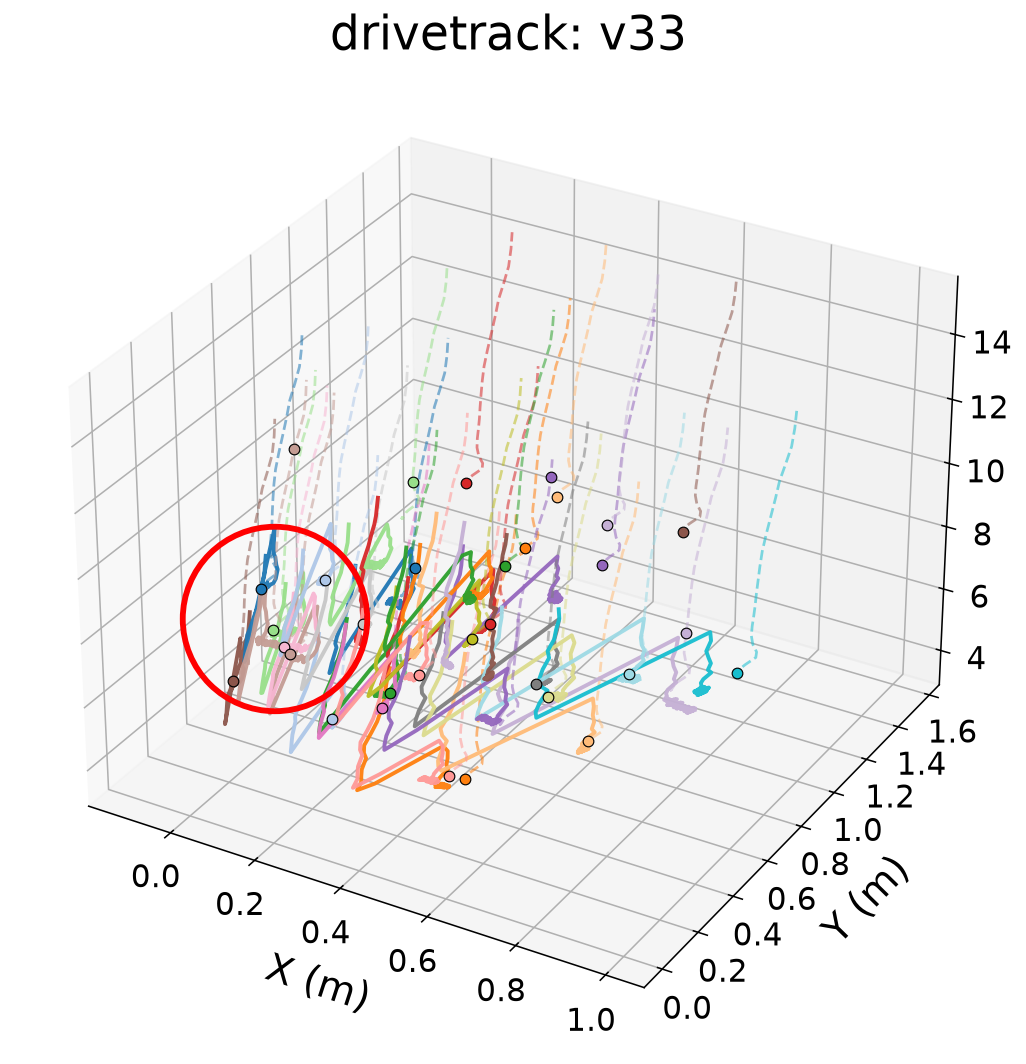
\includegraphics[width=\textwidth]{figs/qual_drivetrack_v33_3d.png}\\{\footnotesize v33}
\end{minipage}
\caption{drivetrack (driving, $\sim$20\,m): the far-field scene where v33's depth correction helps most.}
\label{fig:qual-drivetrack}
\end{figure}

\begin{figure}[h]
\centering
\begin{minipage}{0.49\textwidth}\centering
  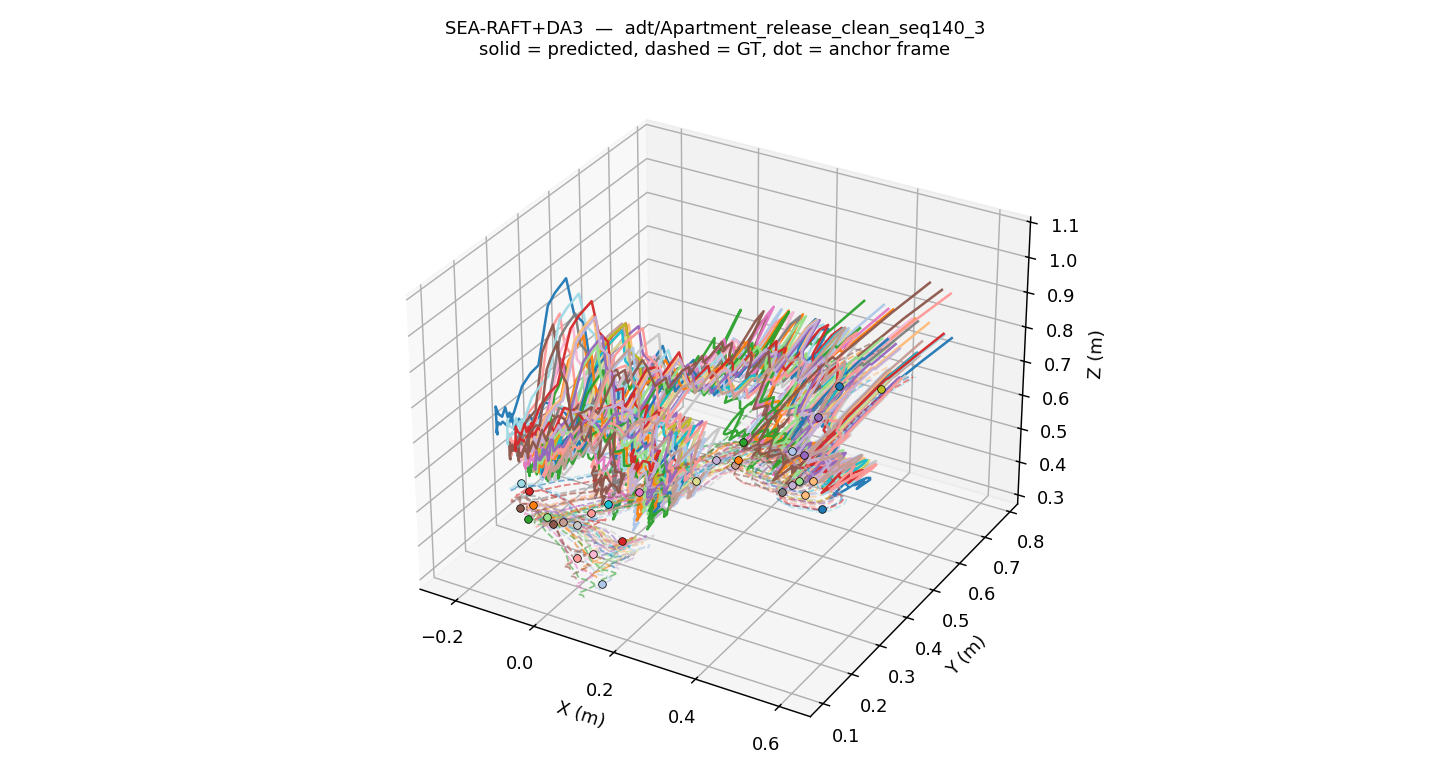
\includegraphics[width=\textwidth]{figs/qual_adt_baseline_3d.png}\\{\footnotesize baseline}
\end{minipage}\hfill
\begin{minipage}{0.49\textwidth}\centering
  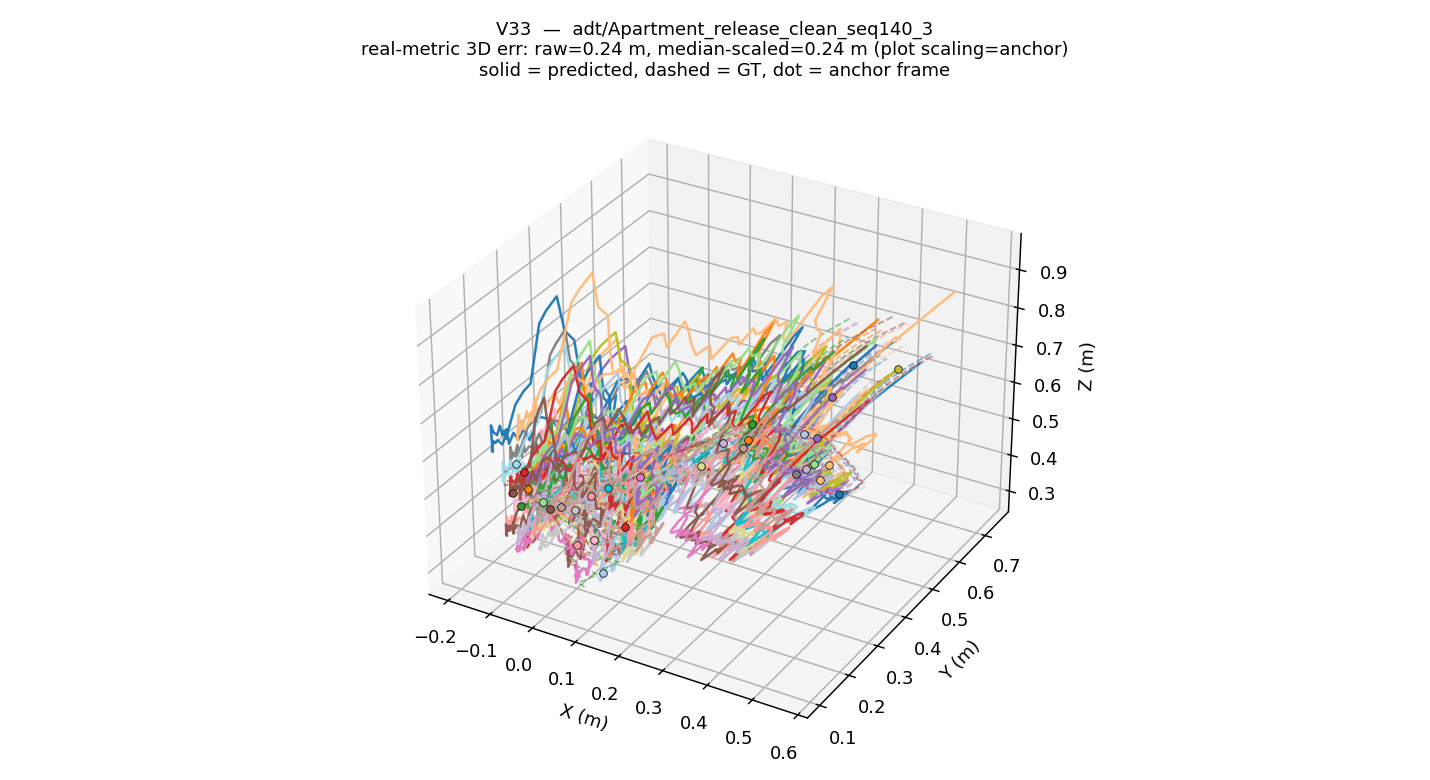
\includegraphics[width=\textwidth]{figs/qual_adt_v33_3d.png}\\{\footnotesize v33}
\end{minipage}
\caption{adt (egocentric, $\sim$1\,m): near-field, where DA3 is already accurate (tie).}
\label{fig:qual-adt}
\end{figure}

\begin{figure}[h]
\centering
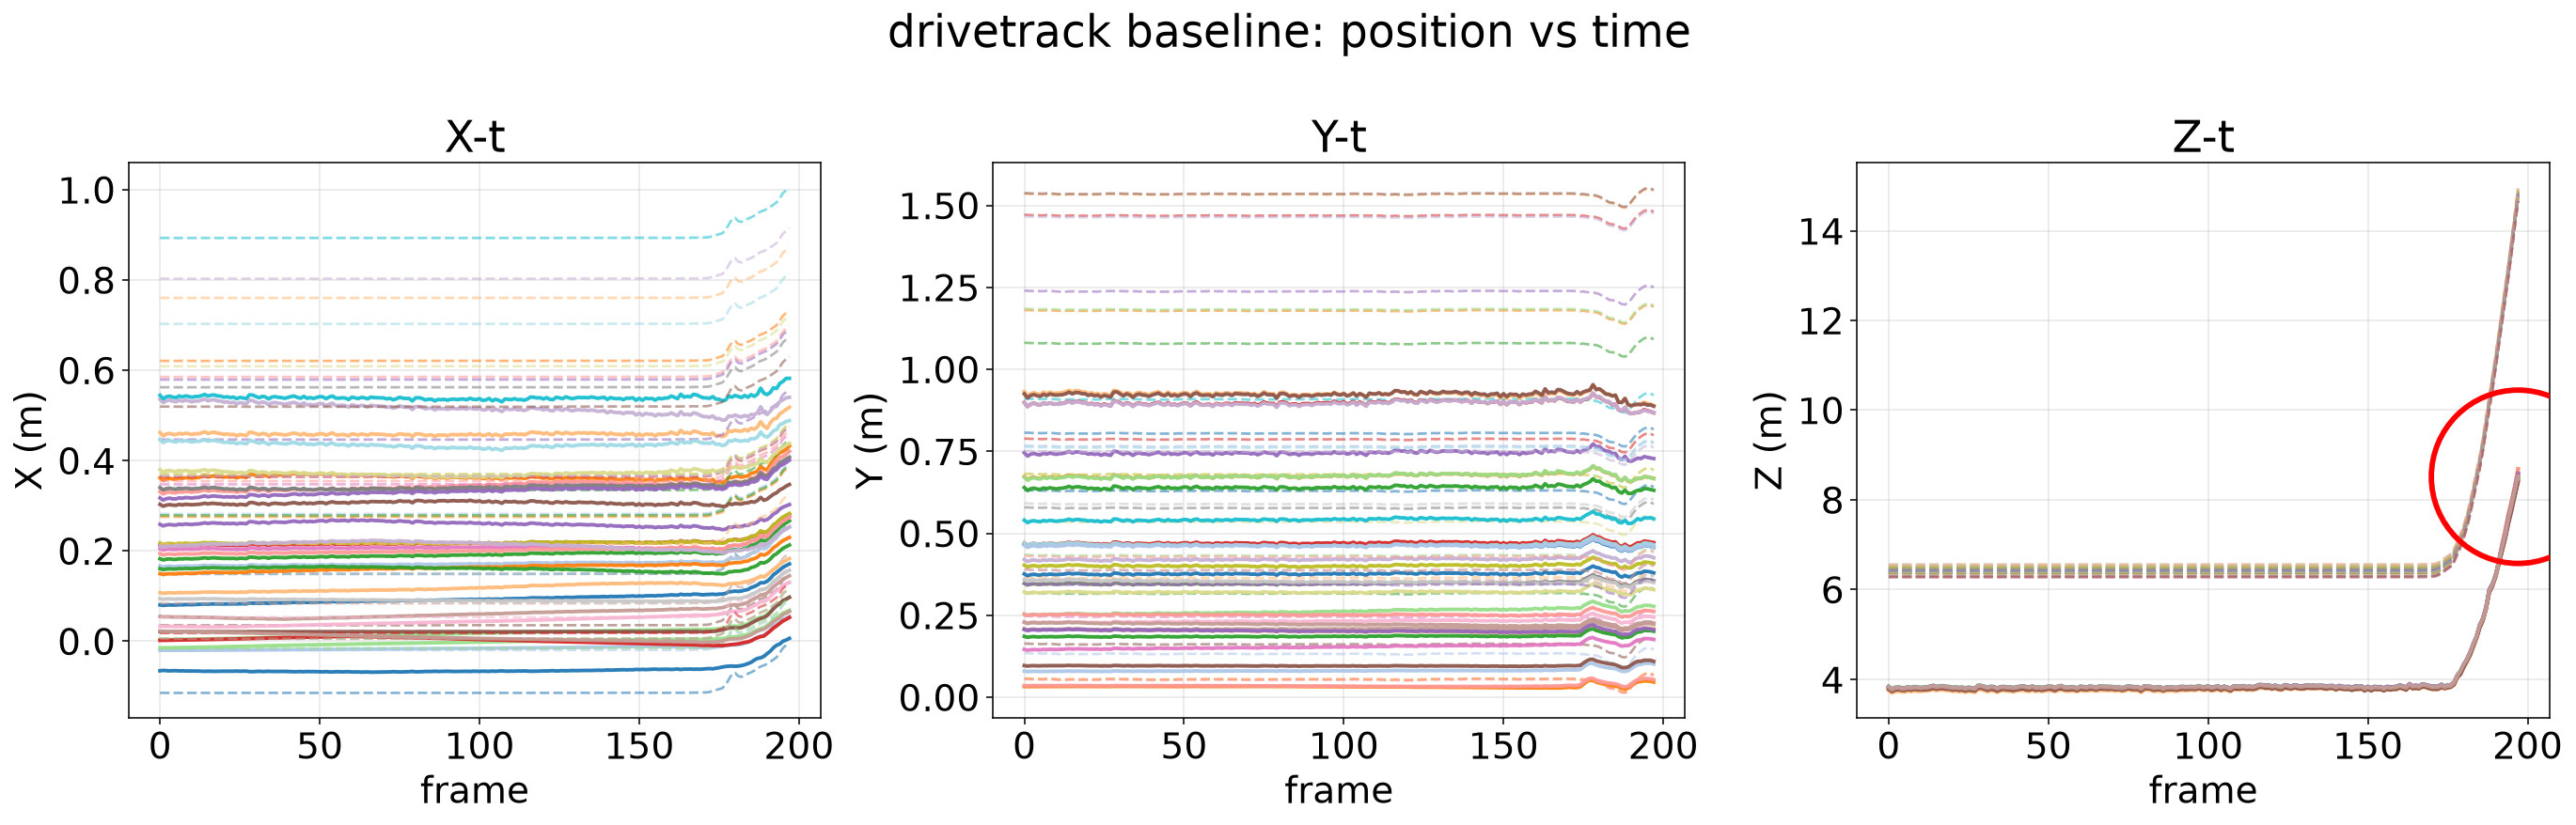
\includegraphics[width=0.92\textwidth]{figs/qual_drivetrack_baseline_st.png}
\caption{Space-time view (drivetrack baseline): per-axis position over time, $X$-$t$/$Y$-$t$/$Z$-$t$,
predicted (solid) vs ground truth (dashed).}
\label{fig:qual-st}
\end{figure}

\subsection{Efficiency}
\begin{table}[h]
\centering
\caption{Inference throughput on RTX\,4080 (12\,GB), measured on TAPVid-3D minival.
         Methods marked $^{\star}$ load depth from a shared DA3-Large precompute
         cache rather than running depth estimation online;
         SpatialTrackerV2 uses its own internal depth model.
         Our lightweight SSM refiner adds modest overhead over the baseline while
         remaining $50$--$200\times$ faster than all competitors.}
\label{tab:efficiency}
\begin{tabular}{lrr}
\toprule
Method & fps & trainable params \\
\midrule
DA3 depth (shared precompute)$^{\star}$ & ${\approx}10$ & 0 \\
\midrule
SEA-RAFT $+$ DA3 (baseline)$^{\star}$  & 12.4 & 0        \\
v33 (depth refiner)$^{\star}$          & 12.5 & 0.40\,M  \\
v35 (DINOv3 $+$ SSM)$^{\star,\dagger}$ & 7.7  & 0.44\,M  \\
v36 (bidir $+$ v35)$^{\star}$          & 6.2  & 0.44\,M  \\
v37 (WAFT $+$ DA3)$^{\star}$           & ${\approx}7.7$ & 0        \\
v39 (WAFT flow $+$ v35)$^{\star}$      & ${\approx}6.3$ & 0.44\,M  \\
\midrule
TAPIP3D$^{\star}$                      & ${\approx}3.1$  & --- \\
SpatialTrackerV2 (s\_wind\,=\,60)      & ${\approx}4.0$  & --- \\
DELTA (DenseTrack3D)$^{\star}$         & ${\approx}7.7$  & --- \\
TrackCraft3R$^{\S}$                    & ${\approx}0.06$ & --- \\
\bottomrule
\end{tabular}
\\[2pt]
{\footnotesize
$^{\star}$ Loads precomputed DA3-Large depth from cache; not counted in fps.
The preprocessing runs at ${\approx}10$\,fps on the same GPU and is a one-time
offline step shared by all such methods.
$^{\dagger}$ v35 throughput measured on the drivetrack subset only.
$^{\S}$ TrackCraft3R is a pre-trained 1.3\,B-parameter video diffusion model (Wan2.1
DiT $+$ 3 VAEs $+$ LoRA); it is not trained by us, hence ``---'' for trainable params.
Throughput measured via windowed inference (see text).}
\end{table}

\paragraph{Why TrackCraft3R is slow.}
TrackCraft3R~\cite{trackcraft3r} adapts Wan2.1-T2V-1.3B --- a video diffusion transformer ---
for 3D tracking via single-step regression.
Each \emph{inference window} (12 frames) requires four sequential GPU passes:
(i)~RGB VAE encode, (ii)~pointmap VAE encode, (iii)~DiT forward through 1.3\,B
parameters, and (iv)~two parallel VAE decodes (xyz $+$ visibility).
The DiT forward alone accounts for ${\approx}75$\,\% of the per-window cost (${\approx}15$--$18$\,s),
with the three VAE passes adding ${\approx}6$\,s; total ${\approx}21$\,s per window on our RTX\,4080.

Critically, each \emph{unique query anchor frame} requires its own window.
TAPVid-3D queries span many frames: a typical 150-frame pstudio clip produces
90--120 unique windows; a 300-frame adt clip produces 260--270 windows.
At 21\,s each, per-clip latency reaches ${\approx}32$\,min (pstudio) and ${\approx}95$\,min (adt),
giving an effective throughput of ${\approx}0.06$\,fps --- \textbf{${\approx}200\times$ slower}
than our baseline (12.4\,fps).

Our method achieves this throughput advantage because the Mamba-3 SSD refiner processes
all $N$ tracks jointly in a single causal sweep per frame (no per-window restarts),
and the 0.44\,M-parameter SSM adds modest overhead over the frozen SEA-RAFT $+$ DA3 baseline.
TAPIP3D (${\approx}3.1$\,fps) and SpatialTrackerV2 (${\approx}4.0$\,fps) are substantially
slower than our pipeline despite relying on simpler (non-diffusion) architectures,
indicating that their multi-frame windowing and cost-volume computations are the bottleneck.
Combined with the accuracy advantage on the absolute metric
(Table~\ref{tab:abs}: mean metric-AJ $0.234$ vs $0.020$ for TrackCraft3R across all three subsets;
see \S\ref{sec:trackcraft3r}),
our pipeline is competitive on both quality and efficiency axes.

% Force all deferred floats before the bibliography
\clearpage
% =====================================================================
\bibliographystyle{unsrt}
\bibliography{refs}

\end{document}
